% Options for packages loaded elsewhere
\PassOptionsToPackage{unicode}{hyperref}
\PassOptionsToPackage{hyphens}{url}
%
\documentclass[
  ngerman,
]{book}
\usepackage{amsmath,amssymb}
\usepackage{lmodern}
\usepackage{iftex}
\ifPDFTeX
  \usepackage[T1]{fontenc}
  \usepackage[utf8]{inputenc}
  \usepackage{textcomp} % provide euro and other symbols
\else % if luatex or xetex
  \usepackage{unicode-math}
  \defaultfontfeatures{Scale=MatchLowercase}
  \defaultfontfeatures[\rmfamily]{Ligatures=TeX,Scale=1}
\fi
% Use upquote if available, for straight quotes in verbatim environments
\IfFileExists{upquote.sty}{\usepackage{upquote}}{}
\IfFileExists{microtype.sty}{% use microtype if available
  \usepackage[]{microtype}
  \UseMicrotypeSet[protrusion]{basicmath} % disable protrusion for tt fonts
}{}
\makeatletter
\@ifundefined{KOMAClassName}{% if non-KOMA class
  \IfFileExists{parskip.sty}{%
    \usepackage{parskip}
  }{% else
    \setlength{\parindent}{0pt}
    \setlength{\parskip}{6pt plus 2pt minus 1pt}}
}{% if KOMA class
  \KOMAoptions{parskip=half}}
\makeatother
\usepackage{xcolor}
\IfFileExists{xurl.sty}{\usepackage{xurl}}{} % add URL line breaks if available
\IfFileExists{bookmark.sty}{\usepackage{bookmark}}{\usepackage{hyperref}}
\hypersetup{
  pdftitle={Computational Statistics},
  pdfauthor={Prof.~Dr.~Dominik Liebl},
  pdflang={de},
  hidelinks,
  pdfcreator={LaTeX via pandoc}}
\urlstyle{same} % disable monospaced font for URLs
\usepackage{color}
\usepackage{fancyvrb}
\newcommand{\VerbBar}{|}
\newcommand{\VERB}{\Verb[commandchars=\\\{\}]}
\DefineVerbatimEnvironment{Highlighting}{Verbatim}{commandchars=\\\{\}}
% Add ',fontsize=\small' for more characters per line
\usepackage{framed}
\definecolor{shadecolor}{RGB}{248,248,248}
\newenvironment{Shaded}{\begin{snugshade}}{\end{snugshade}}
\newcommand{\AlertTok}[1]{\textcolor[rgb]{0.94,0.16,0.16}{#1}}
\newcommand{\AnnotationTok}[1]{\textcolor[rgb]{0.56,0.35,0.01}{\textbf{\textit{#1}}}}
\newcommand{\AttributeTok}[1]{\textcolor[rgb]{0.77,0.63,0.00}{#1}}
\newcommand{\BaseNTok}[1]{\textcolor[rgb]{0.00,0.00,0.81}{#1}}
\newcommand{\BuiltInTok}[1]{#1}
\newcommand{\CharTok}[1]{\textcolor[rgb]{0.31,0.60,0.02}{#1}}
\newcommand{\CommentTok}[1]{\textcolor[rgb]{0.56,0.35,0.01}{\textit{#1}}}
\newcommand{\CommentVarTok}[1]{\textcolor[rgb]{0.56,0.35,0.01}{\textbf{\textit{#1}}}}
\newcommand{\ConstantTok}[1]{\textcolor[rgb]{0.00,0.00,0.00}{#1}}
\newcommand{\ControlFlowTok}[1]{\textcolor[rgb]{0.13,0.29,0.53}{\textbf{#1}}}
\newcommand{\DataTypeTok}[1]{\textcolor[rgb]{0.13,0.29,0.53}{#1}}
\newcommand{\DecValTok}[1]{\textcolor[rgb]{0.00,0.00,0.81}{#1}}
\newcommand{\DocumentationTok}[1]{\textcolor[rgb]{0.56,0.35,0.01}{\textbf{\textit{#1}}}}
\newcommand{\ErrorTok}[1]{\textcolor[rgb]{0.64,0.00,0.00}{\textbf{#1}}}
\newcommand{\ExtensionTok}[1]{#1}
\newcommand{\FloatTok}[1]{\textcolor[rgb]{0.00,0.00,0.81}{#1}}
\newcommand{\FunctionTok}[1]{\textcolor[rgb]{0.00,0.00,0.00}{#1}}
\newcommand{\ImportTok}[1]{#1}
\newcommand{\InformationTok}[1]{\textcolor[rgb]{0.56,0.35,0.01}{\textbf{\textit{#1}}}}
\newcommand{\KeywordTok}[1]{\textcolor[rgb]{0.13,0.29,0.53}{\textbf{#1}}}
\newcommand{\NormalTok}[1]{#1}
\newcommand{\OperatorTok}[1]{\textcolor[rgb]{0.81,0.36,0.00}{\textbf{#1}}}
\newcommand{\OtherTok}[1]{\textcolor[rgb]{0.56,0.35,0.01}{#1}}
\newcommand{\PreprocessorTok}[1]{\textcolor[rgb]{0.56,0.35,0.01}{\textit{#1}}}
\newcommand{\RegionMarkerTok}[1]{#1}
\newcommand{\SpecialCharTok}[1]{\textcolor[rgb]{0.00,0.00,0.00}{#1}}
\newcommand{\SpecialStringTok}[1]{\textcolor[rgb]{0.31,0.60,0.02}{#1}}
\newcommand{\StringTok}[1]{\textcolor[rgb]{0.31,0.60,0.02}{#1}}
\newcommand{\VariableTok}[1]{\textcolor[rgb]{0.00,0.00,0.00}{#1}}
\newcommand{\VerbatimStringTok}[1]{\textcolor[rgb]{0.31,0.60,0.02}{#1}}
\newcommand{\WarningTok}[1]{\textcolor[rgb]{0.56,0.35,0.01}{\textbf{\textit{#1}}}}
\usepackage{longtable,booktabs,array}
\usepackage{calc} % for calculating minipage widths
% Correct order of tables after \paragraph or \subparagraph
\usepackage{etoolbox}
\makeatletter
\patchcmd\longtable{\par}{\if@noskipsec\mbox{}\fi\par}{}{}
\makeatother
% Allow footnotes in longtable head/foot
\IfFileExists{footnotehyper.sty}{\usepackage{footnotehyper}}{\usepackage{footnote}}
\makesavenoteenv{longtable}
\usepackage{graphicx}
\makeatletter
\def\maxwidth{\ifdim\Gin@nat@width>\linewidth\linewidth\else\Gin@nat@width\fi}
\def\maxheight{\ifdim\Gin@nat@height>\textheight\textheight\else\Gin@nat@height\fi}
\makeatother
% Scale images if necessary, so that they will not overflow the page
% margins by default, and it is still possible to overwrite the defaults
% using explicit options in \includegraphics[width, height, ...]{}
\setkeys{Gin}{width=\maxwidth,height=\maxheight,keepaspectratio}
% Set default figure placement to htbp
\makeatletter
\def\fps@figure{htbp}
\makeatother
\setlength{\emergencystretch}{3em} % prevent overfull lines
\providecommand{\tightlist}{%
  \setlength{\itemsep}{0pt}\setlength{\parskip}{0pt}}
\setcounter{secnumdepth}{5}
\usepackage{amsthm}
\usepackage{float}
\usepackage{rotating, graphicx}
\usepackage{multirow}
\usepackage{tabularx}

% new command for pretty oversets with \sim
\newcommand\simcal[1]{\stackrel{\sim}{\smash{\mathcal{#1}}\rule{0pt}{0.5ex}}}

\newcommand{\comma}{,\,}

\floatplacement{figure}{H}

\PassOptionsToPackage{table}{xcolor}

\usepackage{tcolorbox}

\definecolor{kcblue}{HTML}{D7DDEF}
\definecolor{kcdarkblue}{HTML}{2B4E70}

\makeatletter
\def\thm@space@setup{%
  \thm@preskip=8pt plus 2pt minus 4pt
  \thm@postskip=\thm@preskip
}
\makeatother

% \makeatletter % undo the wrong changes made by mathspec
% \let\RequirePackage\original@RequirePackage
% \let\usepackage\RequirePackage
% \makeatother

\newenvironment{rmdknit}
    {\begin{center}
    \begin{tabular}{|p{0.9\textwidth}|}
    \hline\\
    }
    {
    \\\\\hline
    \end{tabular}
    \end{center}
    }

\newenvironment{rmdnote}
    {\begin{center}
    \begin{tabular}{|p{0.9\textwidth}|}
    \hline\\
    }
    {
    \\\\\hline
    \end{tabular}
    \end{center}
    }

\newtcolorbox[auto counter, number within=section]{keyconcepts}[2][]{%
colback=kcblue,colframe=kcdarkblue,fonttitle=\bfseries, title=Key Concept~#2, after title={\newline #1}, beforeafter skip=15pt}

\ifXeTeX
  % Load polyglossia as late as possible: uses bidi with RTL langages (e.g. Hebrew, Arabic)
  \usepackage{polyglossia}
  \setmainlanguage[]{german}
\else
  \usepackage[main=ngerman]{babel}
% get rid of language-specific shorthands (see #6817):
\let\LanguageShortHands\languageshorthands
\def\languageshorthands#1{}
\fi
\ifLuaTeX
  \usepackage{selnolig}  % disable illegal ligatures
\fi
\usepackage[]{natbib}
\bibliographystyle{apalike}

\title{Computational Statistics}
\author{Prof.~Dr.~Dominik Liebl}
\date{}

\begin{document}
\maketitle

{
\setcounter{tocdepth}{1}
\tableofcontents
}
\hypertarget{informationen}{%
\chapter*{Informationen}\label{informationen}}
\addcontentsline{toc}{chapter}{Informationen}

Dies ist das Skript zur Vorlesung \emph{Computational Statistik}

\hypertarget{vorlesungszeiten}{%
\subsection*{Vorlesungszeiten}\label{vorlesungszeiten}}
\addcontentsline{toc}{subsection}{Vorlesungszeiten}

\begin{table}
\centering
\begin{tabular}[t]{l|l|l}
\hline
Wochentag & Uhrzeit & Hörsaal\\
\hline
Dienstag & 9:15-10:45 & Online-Vorlesung\\
\hline
Freitag & 8:30-10:00 & Online-Vorlesung\\
\hline
\end{tabular}
\end{table}

\hypertarget{rcodes}{%
\subsection*{RCodes}\label{rcodes}}
\addcontentsline{toc}{subsection}{RCodes}

Die RCodes zu den einzelnen Kapiteln können hier heruntergeladen werden: \href{https://github.com/lidom/Computational_Statistics_Script/tree/main/RCodes}{RCodes}

\hypertarget{leseecke}{%
\subsection*{Leseecke}\label{leseecke}}
\addcontentsline{toc}{subsection}{Leseecke}

Folgende \emph{frei zugängliche} Lehrbücher enthalten Teile dieses Kurses. In den jeweiligen Kapiteln, werde ich auf die einzelnen Bücher verweisen.

\begin{itemize}
\item
  \href{https://www.microsoft.com/en-us/research/uploads/prod/2006/01/Bishop-Pattern-Recognition-and-Machine-Learning-2006.pdf}{Pattern Recognition and Machine Learning} (by Christopher Bishop)
\item
  \href{https://trevorhastie.github.io/ISLR/}{An Introduction to Statistical Learning, with Applications in R} (by Gareth James, Daniela Witten, Trevor Hastie and Robert Tibshirani).
\item
  \href{https://web.stanford.edu/~hastie/StatLearnSparsity/}{Statistical Learning with Sparsity: the Lasso and Generalizations} (by Trevor Hastie, Robert Tibshirani and Martin Wainwright).
\item
  \href{https://web.stanford.edu/~hastie/ElemStatLearn/}{Elements of Statistical Learning: Data mining, Inference and Prediction} (by Trevor Hastie, Robert Tibshirani and Jerome Friedman).
\item
  \href{https://web.stanford.edu/~hastie/CASI/}{Computer Age Statistical Inference: Algorithms, Evidence and Data Science} (by Bradley Efron and Trevor Hastie)
\end{itemize}

\hypertarget{florence-nightingale}{%
\subsection*{Florence Nightingale}\label{florence-nightingale}}
\addcontentsline{toc}{subsection}{Florence Nightingale}

Das Logo zu diesem Skript stammt von einer \href{https://de.wikipedia.org/wiki/Datei:DBP_1955_225_Florence_Nightingale.jpg}{Briefmarke} zur Erinnerung an die Krankenschwester und \href{https://infowetrust.com/project/designhero}{inspirierende Statistikerin}, \href{https://de.wikipedia.org/wiki/Florence_Nightingale}{Florence Nightingale}. Nightingale war die Begründerin der modernen westlichen Krankenpflege und Pionierin der \href{https://de.wikipedia.org/wiki/Kreisdiagramm\#/media/Datei:Nightingale-mortality.jpg}{visuellen Datenanalyse}. Sie nutzte statistische Analysen, um Missstände in Kliniken zu erkennen und diese dann auch nachweislich abzustellen. Sie ist die erste Frau, die in die britische \href{https://rss.org.uk/}{Royal Statistical Society} aufgenommen wurde; später erhielt sie auch die Ehrenmitgliedschaft der \href{https://www.amstat.org/}{American Statistical Association}.

\hypertarget{der-expectation-maximization-em-algorithmus}{%
\chapter{Der Expectation Maximization (EM) Algorithmus}\label{der-expectation-maximization-em-algorithmus}}

Der EM Algorithmus wird häufig verwendet, um komplizierte Maximum Likelihood Schätzprobleme zu vereinfachen bzw. überhaupt erst möglich zu machen. In diesem Kapitel stellen wir den EM Algorithmus zur Schätzung von Gaußschen Mischverteilungen vor, da der EM Algorithmus hier wohl seine bekannteste Anwendung hat. Bereits die originale Arbeit zum EM Algorithmus \citep{Dempster_1977} beschäftigt sich mit der Schätzung von Gaußschen Mischverteilungen.

\textbf{Mögliche Anwendungen von Gaußschen Mischverteilungen:}

\begin{itemize}
\item
  Generell: Auffinden von Gruppierungen (zwei oder mehr) in den Daten (\textbf{Clusteranalyse}). Zum Beispiel:

  \begin{itemize}
  \tightlist
  \item
    Automatisierte Videobearbeitungen (z.B. Bildeinteilungen in Vorder- und Hintergrund)
  \item
    Automatisierte Erkennung von Laufstilen
  \item
    etc.
  \end{itemize}
\end{itemize}

\hypertarget{lernziele-fuxfcr-dieses-kapitel}{%
\subsection*{Lernziele für dieses Kapitel}\label{lernziele-fuxfcr-dieses-kapitel}}
\addcontentsline{toc}{subsection}{Lernziele für dieses Kapitel}

Sie können \ldots{}

\begin{itemize}
\tightlist
\item
  ein \textbf{Anwendungsfeld} des EM Algorithmuses \textbf{benennen}.
\item
  die \textbf{Probleme} der klassischen Maximum Likelihood Methode zur Schätzung von Gaußschen Mischverteilungen \textbf{benennen und erläutern}.
\item
  die \textbf{Grundidee} des EM Algorithmuses \textbf{erläutern}.
\item
  den \textbf{EM Algorithmus} zur Schätzung von Gaußschen Mischverteilungen \textbf{anwenden}.
\item
  die \textbf{Grundidee} der Vervollständigung der Daten durch latente Variablen \textbf{erläutern}.
\end{itemize}

\hypertarget{begleitlektuxfcren}{%
\subsection*{Begleitlektüre(n)}\label{begleitlektuxfcren}}
\addcontentsline{toc}{subsection}{Begleitlektüre(n)}

Zur Vorbereitung der Klausur ist es grundsätzlich aussreichend dieses Kapitel durchzuarbeiten - aber Lesen hat ja noch nie geschadet. Dieses Kapitel basiert hauptsächlich auf:

\begin{itemize}
\tightlist
\item
  Kapitel 9 in \href{https://www.microsoft.com/en-us/research/uploads/prod/2006/01/Bishop-Pattern-Recognition-and-Machine-Learning-2006.pdf}{\textbf{Pattern Recognition and Machine Learning}} \citep{book_Bishop2006}.
  Die pdf-Version des Buches ist frei erhältlichen: \href{https://www.microsoft.com/en-us/research/uploads/prod/2006/01/Bishop-Pattern-Recognition-and-Machine-Learning-2006.pdf}{\textbf{pdf-Version}}
\end{itemize}

Weiteren guten Lesestoff zum EM Algoithmus gibt es z.B. hier:

\begin{itemize}
\tightlist
\item
  Kapitel 8.5 in \href{https://web.stanford.edu/~hastie/ElemStatLearn/}{\textbf{Elements of Statistical Learning: Data Mining, Inference and Prediction}} \citep{Elements}.
  Die pdf-Version des Buches ist frei erhältlichen: \href{https://web.stanford.edu/~hastie/ElemStatLearn/}{\textbf{pdf-Version}}
\end{itemize}

\hypertarget{r-pakete-fuxfcr-diese-kapitel}{%
\subsection*{R-Pakete für diese Kapitel}\label{r-pakete-fuxfcr-diese-kapitel}}
\addcontentsline{toc}{subsection}{R-Pakete für diese Kapitel}

Folgende R-Pakete werden für dieses Kapitel benötigt:

\begin{Shaded}
\begin{Highlighting}[]
\NormalTok{pkgs }\OtherTok{\textless{}{-}} \FunctionTok{c}\NormalTok{(}\StringTok{"tidyverse"}\NormalTok{,      }\CommentTok{\# Die tidyverse{-}Pakete}
          \StringTok{"palmerpenguins"}\NormalTok{, }\CommentTok{\# Pinguin{-}Daten}
          \StringTok{"scales"}\NormalTok{,         }\CommentTok{\# Transparente Farben: alpha()}
          \StringTok{"RColorBrewer"}\NormalTok{,   }\CommentTok{\# Hübsche Farben}
          \StringTok{"mclust"}\NormalTok{,         }\CommentTok{\# Schätzung/Verwendung }
                            \CommentTok{\# Gaußschen Mischverteilungen}
          \StringTok{"MASS"}\NormalTok{)           }\CommentTok{\# Erzeugung von Zufallszahlen aus }
                            \CommentTok{\# einer multiv. Normalverteilung}
\FunctionTok{install.packages}\NormalTok{(pkgs)}
\end{Highlighting}
\end{Shaded}

\hypertarget{motivation-clusteranalyse-mit-hilfe-gauuxdfscher-mischverteilungen}{%
\section{Motivation: Clusteranalyse mit Hilfe Gaußscher Mischverteilungen}\label{motivation-clusteranalyse-mit-hilfe-gauuxdfscher-mischverteilungen}}

Als Datenbeispiel verwendent wir die \href{https://allisonhorst.github.io/palmerpenguins/articles/intro.html}{\texttt{palmerpenguins}} Daten \citep{palmerpenguins}.

Diese Daten stammen aus Vermessungen von Pinguinpopulationen auf dem Palmer-Archipel (Antarktische Halbinsel). Pinguine sind oft schwer von einander zu unterscheiden. Wir werden versuchen, mit Hilfe einer Gaußschen Mischverteilung Gruppierungen in den Pinguindaten (Flossenlänge) zu finden. Um solche Mischverteilungen schätzen zu können, führen wir den EM Algorithmus ein.

Der folgende Code-Chunck bereitet die Daten auf.

\begin{quote}
\textbf{Achtung:} Wir haben zwar die Information zu den verschiedenen Pinguin-Arten (\texttt{Penguine\_Art}) tun aber im Folgenden so, also ob wir diese Information nicht kennen würden. Wir wollen alleine auf Basis der Flossenlängen (\texttt{Penguine\_Flosse}) die Gruppenzugehörigkeiten per Clusteranalyse bestimmen. (Im Nachhinein können wir dann mit Hilfe der Daten in \texttt{Penguine\_Art} prüfen, wie gut unsere Clusteranalyse ist.)
\end{quote}

\begin{Shaded}
\begin{Highlighting}[]
\FunctionTok{library}\NormalTok{(}\StringTok{"palmerpenguins"}\NormalTok{) }\CommentTok{\# Pinguin{-}Daten}
\FunctionTok{library}\NormalTok{(}\StringTok{"RColorBrewer"}\NormalTok{)   }\CommentTok{\# Hübsche Farben}
\FunctionTok{library}\NormalTok{(}\StringTok{"scales"}\NormalTok{)         }\CommentTok{\# Für transparente Farben: alpha()}

\NormalTok{col\_v }\OtherTok{\textless{}{-}}\NormalTok{ RColorBrewer}\SpecialCharTok{::}\FunctionTok{brewer.pal}\NormalTok{(}\AttributeTok{n =} \DecValTok{3}\NormalTok{, }\AttributeTok{name =} \StringTok{"Set2"}\NormalTok{)}

\DocumentationTok{\#\# Vorbereitung der Daten:}
\NormalTok{Pinguine }\OtherTok{\textless{}{-}}\NormalTok{ palmerpenguins}\SpecialCharTok{::}\NormalTok{penguins }\SpecialCharTok{\%\textgreater{}\%} \CommentTok{\# Pinguin{-}Daten}
\NormalTok{  tidyr}\SpecialCharTok{::}\FunctionTok{as\_tibble}\NormalTok{() }\SpecialCharTok{\%\textgreater{}\%}                 \CommentTok{\# Datenformat: \textquotesingle{}tibble\textquotesingle{}{-}dataframe}
\NormalTok{  dplyr}\SpecialCharTok{::}\FunctionTok{filter}\NormalTok{(species}\SpecialCharTok{!=}\StringTok{"Adelie"}\NormalTok{) }\SpecialCharTok{\%\textgreater{}\%}   \CommentTok{\# Pinguin{-}Art \textquotesingle{}Adelie\textquotesingle{} löschen }
  \FunctionTok{droplevels}\NormalTok{() }\SpecialCharTok{\%\textgreater{}\%}                       \CommentTok{\# Lösche das nicht mehr benötigte Adelie{-}Level}
\NormalTok{  tidyr}\SpecialCharTok{::}\FunctionTok{drop\_na}\NormalTok{() }\SpecialCharTok{\%\textgreater{}\%}                   \CommentTok{\# NAs löschen}
\NormalTok{  dplyr}\SpecialCharTok{::}\FunctionTok{mutate}\NormalTok{(}\AttributeTok{Art    =}\NormalTok{ species,        }\CommentTok{\# Variablen umbenennen}
                \AttributeTok{Flosse =}\NormalTok{ flipper\_length\_mm) }\SpecialCharTok{\%\textgreater{}\%} 
\NormalTok{  dplyr}\SpecialCharTok{::}\FunctionTok{select}\NormalTok{(Art, Flosse)             }\CommentTok{\# Variablen auswählen}

\DocumentationTok{\#\#  }
\NormalTok{n      }\OtherTok{\textless{}{-}} \FunctionTok{nrow}\NormalTok{(Pinguine)                 }\CommentTok{\# Stichprobenumfang}

\DocumentationTok{\#\# Variable \textquotesingle{}Penguine\_Art\textquotesingle{} aus Pinguine{-}Daten "herausziehen"}
\NormalTok{Penguine\_Art    }\OtherTok{\textless{}{-}}\NormalTok{ dplyr}\SpecialCharTok{::}\FunctionTok{pull}\NormalTok{(Pinguine, Art)}

\DocumentationTok{\#\# Variable \textquotesingle{}Penguine\_Flosse\textquotesingle{} aus Pinguine{-}Daten "herausziehen"}
\NormalTok{Penguine\_Flosse }\OtherTok{\textless{}{-}}\NormalTok{ dplyr}\SpecialCharTok{::}\FunctionTok{pull}\NormalTok{(Pinguine, Flosse)}

\DocumentationTok{\#\# Plot}
\DocumentationTok{\#\# Histogramm:}
\FunctionTok{hist}\NormalTok{(}\AttributeTok{x =}\NormalTok{ Penguine\_Flosse, }\AttributeTok{freq =} \ConstantTok{FALSE}\NormalTok{, }
     \AttributeTok{xlab=}\StringTok{"Flossenlänge (mm)"}\NormalTok{, }\AttributeTok{main=}\StringTok{"Pinguine}\SpecialCharTok{\textbackslash{}n}\StringTok{(Zwei Gruppen)"}\NormalTok{,}
     \AttributeTok{col=}\FunctionTok{gray}\NormalTok{(.}\DecValTok{65}\NormalTok{,.}\DecValTok{5}\NormalTok{), }\AttributeTok{border=}\FunctionTok{gray}\NormalTok{(.}\DecValTok{35}\NormalTok{,.}\DecValTok{5}\NormalTok{), }\AttributeTok{ylim=}\FunctionTok{c}\NormalTok{(}\FloatTok{0.0003}\NormalTok{, }\FloatTok{0.039}\NormalTok{))}
\DocumentationTok{\#\# Stipchart hinzufügen:}
\FunctionTok{stripchart}\NormalTok{(}\AttributeTok{x =}\NormalTok{ Penguine\_Flosse, }\AttributeTok{method =} \StringTok{"jitter"}\NormalTok{, }
           \AttributeTok{jitter =}\NormalTok{ .}\DecValTok{0005}\NormalTok{, }\AttributeTok{at =}\NormalTok{ .}\DecValTok{001}\NormalTok{,}
           \AttributeTok{pch =} \DecValTok{21}\NormalTok{, }\AttributeTok{col=}\FunctionTok{alpha}\NormalTok{(col\_v[}\DecValTok{3}\NormalTok{],.}\DecValTok{5}\NormalTok{), }
           \AttributeTok{bg=}\FunctionTok{alpha}\NormalTok{(col\_v[}\DecValTok{3}\NormalTok{],.}\DecValTok{5}\NormalTok{), }\AttributeTok{cex=}\FloatTok{1.3}\NormalTok{, }\AttributeTok{add =} \ConstantTok{TRUE}\NormalTok{)}
\end{Highlighting}
\end{Shaded}

\begin{center}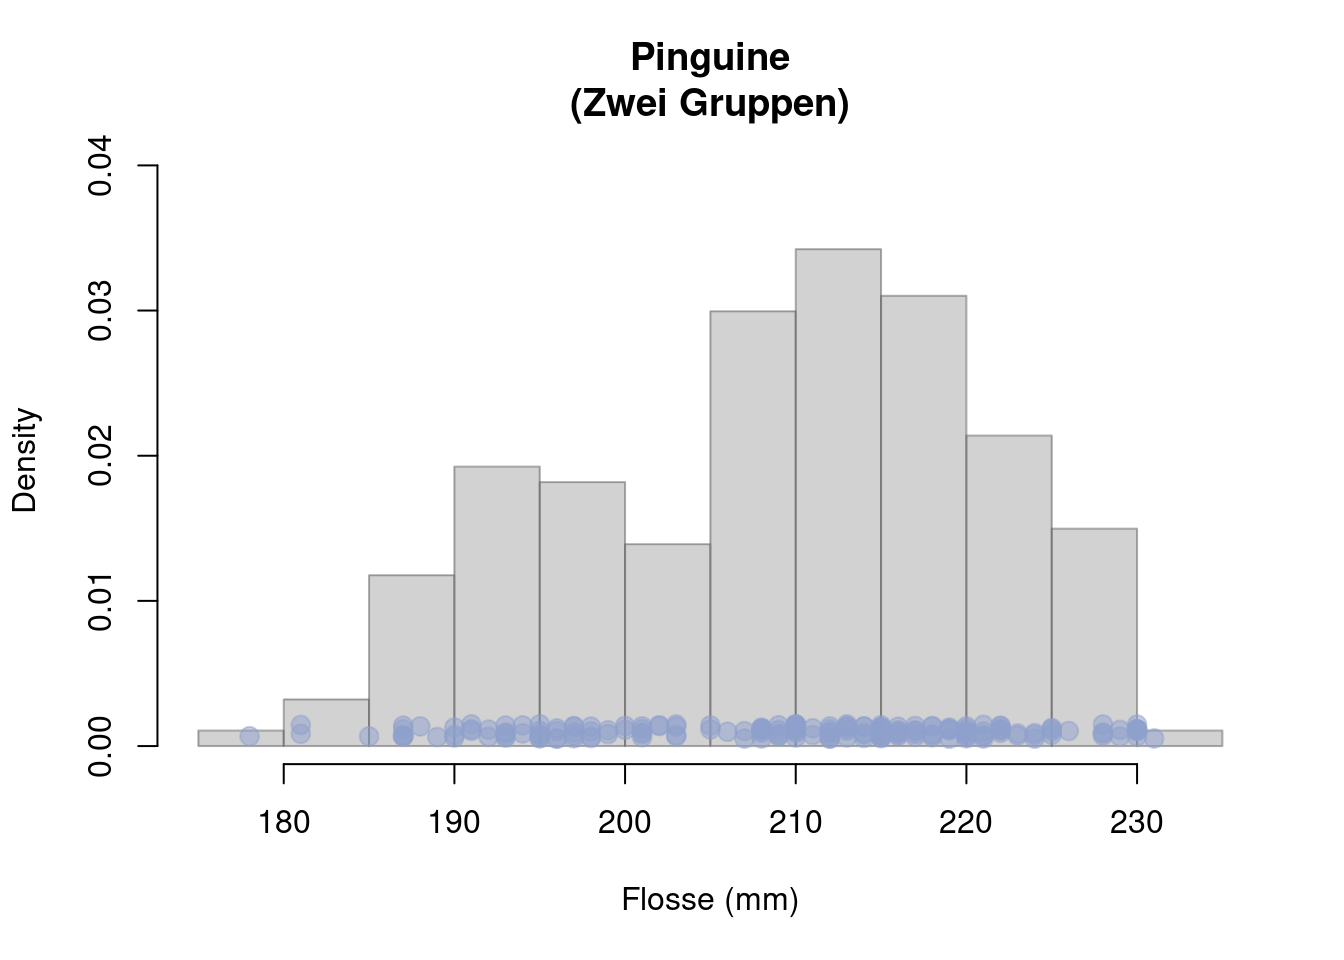
\includegraphics[width=1\linewidth]{Computational_Statistics_Script_files/figure-latex/unnamed-chunk-9-1} \end{center}

\textbf{Das Clusterverfahren basierend auf Gaußschen Mischverteilungen:}

\begin{enumerate}
\def\labelenumi{\arabic{enumi}.}
\tightlist
\item
  Gaußsche Mischverteilung (\textbf{per EM Algorithmus}) schätzen
\item
  Die Datenpunkte \(x_i\) derjenigen Gruppe zuordnen, welche die \textbf{„a-posteriori-Wahrscheinlichkeit``} maximiert (siehe Abbildung \ref{fig:GMM-plot1})
\end{enumerate}

\begin{figure}[h]

{\centering 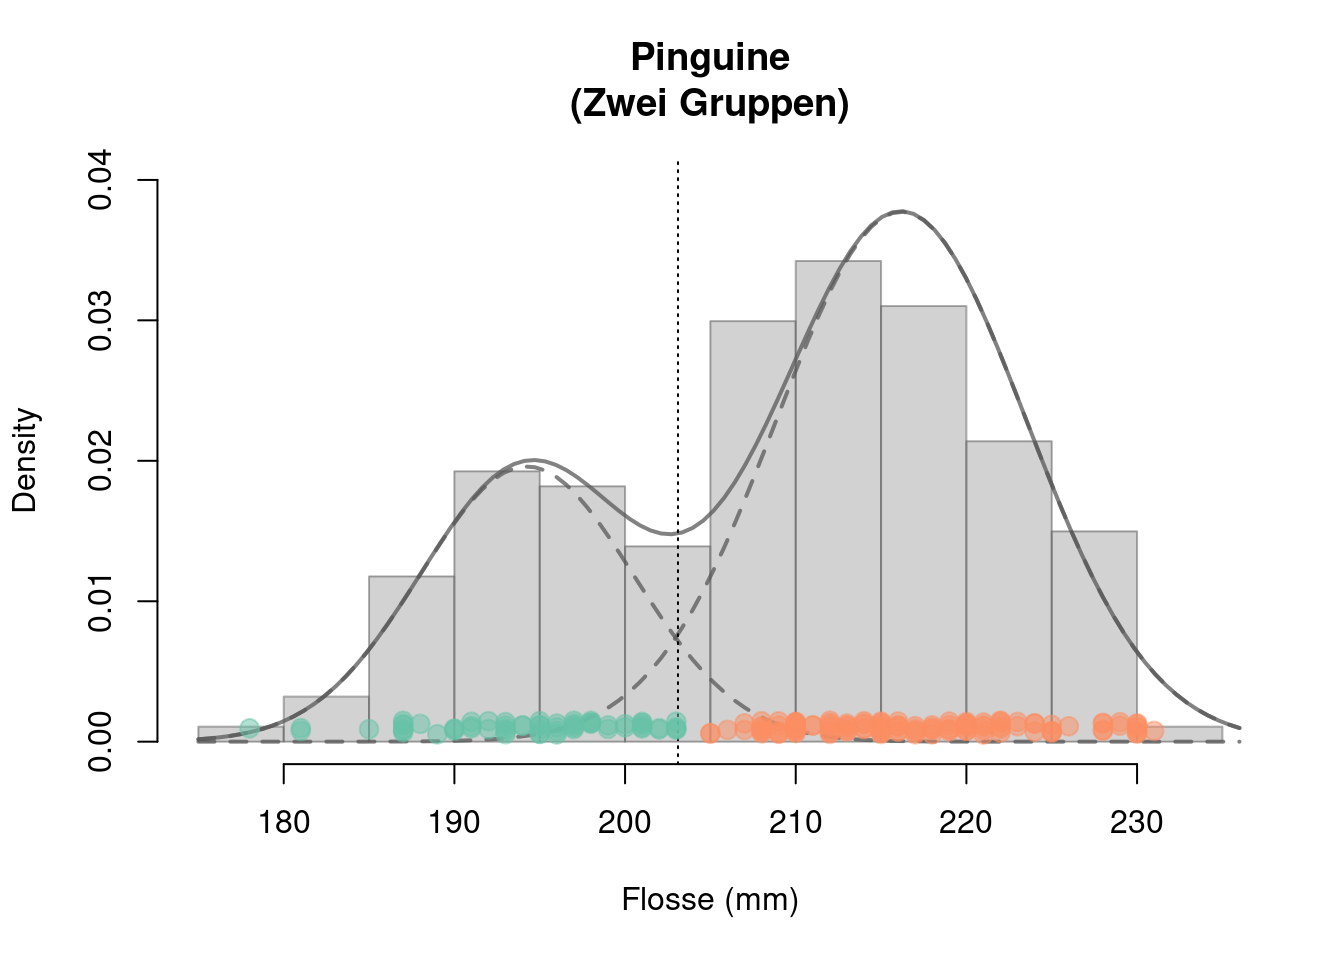
\includegraphics[width=1\linewidth]{Computational_Statistics_Script_files/figure-latex/GMM-plot1-1} 

}

\caption{Clusteranalyse basierend auf einer  Mischverteilung mit zwei gewichteten Normalverteilungen.}\label{fig:GMM-plot1}
\end{figure}

Abbildung \ref{fig:GMM-plot1} zeigt das Resultat einer Clusteranalyse basierend auf einer Mischverteilung zweier gewichteter Normalverteilungen. Cluster-Ergebnis: 95\% der Pinguine konnten richtig zugeordnet werden - lediglich auf Basis ihrer Flossenlängen.

Mit Hilfe der folgenden R-Codes kann die obige Clusteranalyse und die Ergebnisgrafik repliziert werden:

\begin{Shaded}
\begin{Highlighting}[]
\DocumentationTok{\#\# mclust R{-}Paket:}
\DocumentationTok{\#\# Clusteranalyse mit Hilfe von Gaußschen Mischmodellen}
\FunctionTok{suppressMessages}\NormalTok{(}\FunctionTok{library}\NormalTok{(}\StringTok{"mclust"}\NormalTok{))}

\DocumentationTok{\#\# Anzahl der Gruppen}
\NormalTok{G }\OtherTok{\textless{}{-}} \DecValTok{2} 

\DocumentationTok{\#\# Schätzung des Gaußschen Mischmodells (per EM Algorithmus)}
\DocumentationTok{\#\# und Clusteranalyse}
\NormalTok{mclust\_obj }\OtherTok{\textless{}{-}}\NormalTok{ mclust}\SpecialCharTok{::}\FunctionTok{Mclust}\NormalTok{(}\AttributeTok{data =}\NormalTok{ Penguine\_Flosse, }\AttributeTok{G=}\NormalTok{G, }
                              \AttributeTok{modelNames =} \StringTok{"V"}\NormalTok{, }
                              \AttributeTok{verbose =} \ConstantTok{FALSE}\NormalTok{)}

\CommentTok{\# summary(mclust\_obj)}
\CommentTok{\# str(mclust\_obj)}

\DocumentationTok{\#\# Geschätzte Gruppen{-}Zuordnungen (Cluster{-}Resultat)}
\NormalTok{class }\OtherTok{\textless{}{-}}\NormalTok{ mclust\_obj}\SpecialCharTok{$}\NormalTok{classification}

\DocumentationTok{\#\# Anteil der korrekten Zuordnungen:}
\CommentTok{\# cbind(class, Penguine\_Art)}
\FunctionTok{round}\NormalTok{(}\FunctionTok{sum}\NormalTok{(class }\SpecialCharTok{==} \FunctionTok{as.numeric}\NormalTok{(Penguine\_Art))}\SpecialCharTok{/}\NormalTok{n, }\DecValTok{2}\NormalTok{)}

\DocumentationTok{\#\# Geschätzte Mittelwerte }
\NormalTok{mean\_m }\OtherTok{\textless{}{-}} \FunctionTok{t}\NormalTok{(mclust\_obj}\SpecialCharTok{$}\NormalTok{parameters}\SpecialCharTok{$}\NormalTok{mean)}

\DocumentationTok{\#\# Geschätzte Varianzen (und evtl. Kovarianzen) }
\NormalTok{cov\_l  }\OtherTok{\textless{}{-}} \FunctionTok{list}\NormalTok{(}\StringTok{"Cov1"} \OtherTok{=}\NormalTok{ mclust\_obj}\SpecialCharTok{$}\NormalTok{parameters}\SpecialCharTok{$}\NormalTok{variance}\SpecialCharTok{$}\NormalTok{sigmasq[}\DecValTok{1}\NormalTok{], }
               \StringTok{"Cov2"} \OtherTok{=}\NormalTok{ mclust\_obj}\SpecialCharTok{$}\NormalTok{parameters}\SpecialCharTok{$}\NormalTok{variance}\SpecialCharTok{$}\NormalTok{sigmasq[}\DecValTok{2}\NormalTok{])}

\DocumentationTok{\#\# Geschätzte Gewichte (a{-}priori{-}Wahrscheinlichkeiten) }
\NormalTok{prop\_v }\OtherTok{\textless{}{-}}\NormalTok{ mclust\_obj}\SpecialCharTok{$}\NormalTok{parameters}\SpecialCharTok{$}\NormalTok{pro}

\DocumentationTok{\#\# Auswerten der Gaußsche Mischung{-}Dichtefunktion}
\NormalTok{np      }\OtherTok{\textless{}{-}} \DecValTok{100} \CommentTok{\# Anzahl der Auswertungspunkte}
\NormalTok{xxd     }\OtherTok{\textless{}{-}} \FunctionTok{seq}\NormalTok{(}\FunctionTok{min}\NormalTok{(Penguine\_Flosse)}\SpecialCharTok{{-}}\DecValTok{3}\NormalTok{, }\FunctionTok{max}\NormalTok{(Penguine\_Flosse)}\SpecialCharTok{+}\DecValTok{5}\NormalTok{, }\AttributeTok{length.out =}\NormalTok{ np)}
\DocumentationTok{\#\# Mischungs{-}Dichte}
\NormalTok{yyd     }\OtherTok{\textless{}{-}} \FunctionTok{dnorm}\NormalTok{(xxd, mean\_m[}\DecValTok{1}\NormalTok{], }\FunctionTok{sqrt}\NormalTok{(cov\_l[[}\DecValTok{1}\NormalTok{]]))}\SpecialCharTok{*}\NormalTok{prop\_v[}\DecValTok{1}\NormalTok{] }\SpecialCharTok{+}
           \FunctionTok{dnorm}\NormalTok{(xxd, mean\_m[}\DecValTok{2}\NormalTok{], }\FunctionTok{sqrt}\NormalTok{(cov\_l[[}\DecValTok{2}\NormalTok{]]))}\SpecialCharTok{*}\NormalTok{prop\_v[}\DecValTok{2}\NormalTok{]}
\DocumentationTok{\#\# Einzel{-}Dichten}
\NormalTok{yyd1    }\OtherTok{\textless{}{-}} \FunctionTok{dnorm}\NormalTok{(xxd, mean\_m[}\DecValTok{1}\NormalTok{], }\FunctionTok{sqrt}\NormalTok{(cov\_l[[}\DecValTok{1}\NormalTok{]]))}\SpecialCharTok{*}\NormalTok{prop\_v[}\DecValTok{1}\NormalTok{]}
\NormalTok{yyd2    }\OtherTok{\textless{}{-}} \FunctionTok{dnorm}\NormalTok{(xxd, mean\_m[}\DecValTok{2}\NormalTok{], }\FunctionTok{sqrt}\NormalTok{(cov\_l[[}\DecValTok{2}\NormalTok{]]))}\SpecialCharTok{*}\NormalTok{prop\_v[}\DecValTok{2}\NormalTok{]}

\DocumentationTok{\#\# Plot}
\FunctionTok{hist}\NormalTok{(}\AttributeTok{x =}\NormalTok{ Penguine\_Flosse, }\AttributeTok{xlab=}\StringTok{"Flossenlänge (mm)"}\NormalTok{, }\AttributeTok{main=}\StringTok{"Pinguine}\SpecialCharTok{\textbackslash{}n}\StringTok{(Zwei Gruppen)"}\NormalTok{,}
     \AttributeTok{col=}\FunctionTok{gray}\NormalTok{(.}\DecValTok{65}\NormalTok{,.}\DecValTok{5}\NormalTok{), }\AttributeTok{border=}\FunctionTok{gray}\NormalTok{(.}\DecValTok{35}\NormalTok{,.}\DecValTok{5}\NormalTok{), }\AttributeTok{freq =} \ConstantTok{FALSE}\NormalTok{, }\AttributeTok{ylim=}\FunctionTok{c}\NormalTok{(}\DecValTok{0}\NormalTok{, }\FloatTok{0.04}\NormalTok{))}
\FunctionTok{lines}\NormalTok{(}\AttributeTok{x =}\NormalTok{ xxd, }\AttributeTok{y=}\NormalTok{yyd, }\AttributeTok{lwd=}\DecValTok{2}\NormalTok{, }\AttributeTok{col=}\FunctionTok{gray}\NormalTok{(.}\DecValTok{35}\NormalTok{,.}\DecValTok{75}\NormalTok{))}
\FunctionTok{lines}\NormalTok{(}\AttributeTok{x =}\NormalTok{ xxd, }\AttributeTok{y=}\NormalTok{yyd1, }\AttributeTok{lwd=}\DecValTok{2}\NormalTok{, }\AttributeTok{col=}\FunctionTok{gray}\NormalTok{(.}\DecValTok{35}\NormalTok{,.}\DecValTok{75}\NormalTok{), }\AttributeTok{lty=}\DecValTok{2}\NormalTok{)}
\FunctionTok{lines}\NormalTok{(}\AttributeTok{x =}\NormalTok{ xxd, }\AttributeTok{y=}\NormalTok{yyd2, }\AttributeTok{lwd=}\DecValTok{2}\NormalTok{, }\AttributeTok{col=}\FunctionTok{gray}\NormalTok{(.}\DecValTok{35}\NormalTok{,.}\DecValTok{75}\NormalTok{), }\AttributeTok{lty=}\DecValTok{2}\NormalTok{)}
\FunctionTok{stripchart}\NormalTok{(Penguine\_Flosse[class}\SpecialCharTok{==}\DecValTok{1}\NormalTok{], }\AttributeTok{method =} \StringTok{"jitter"}\NormalTok{, }\AttributeTok{jitter =}\NormalTok{ .}\DecValTok{0005}\NormalTok{, }\AttributeTok{at =}\NormalTok{ .}\DecValTok{001}\NormalTok{,}
           \AttributeTok{pch =} \DecValTok{21}\NormalTok{, }\AttributeTok{col=}\FunctionTok{alpha}\NormalTok{(col\_v[}\DecValTok{1}\NormalTok{],.}\DecValTok{5}\NormalTok{), }\AttributeTok{bg=}\FunctionTok{alpha}\NormalTok{(col\_v[}\DecValTok{1}\NormalTok{],.}\DecValTok{5}\NormalTok{), }\AttributeTok{cex=}\FloatTok{1.3}\NormalTok{, }\AttributeTok{add =} \ConstantTok{TRUE}\NormalTok{)}
\FunctionTok{stripchart}\NormalTok{(Penguine\_Flosse[class}\SpecialCharTok{==}\DecValTok{2}\NormalTok{], }\AttributeTok{method =} \StringTok{"jitter"}\NormalTok{, }\AttributeTok{jitter =}\NormalTok{ .}\DecValTok{0005}\NormalTok{, }\AttributeTok{at =}\NormalTok{ .}\DecValTok{001}\NormalTok{,}
           \AttributeTok{pch =} \DecValTok{21}\NormalTok{, }\AttributeTok{col=}\FunctionTok{alpha}\NormalTok{(col\_v[}\DecValTok{2}\NormalTok{],.}\DecValTok{5}\NormalTok{), }\AttributeTok{bg=}\FunctionTok{alpha}\NormalTok{(col\_v[}\DecValTok{2}\NormalTok{],.}\DecValTok{5}\NormalTok{), }\AttributeTok{cex=}\FloatTok{1.3}\NormalTok{, }\AttributeTok{add =} \ConstantTok{TRUE}\NormalTok{)}
\end{Highlighting}
\end{Shaded}

\hypertarget{der-em-algorithmus-zur-ml-schuxe4tzung-gauuxdfscher-mischverteilungen}{%
\section{Der EM Algorithmus zur ML-Schätzung Gaußscher Mischverteilungen}\label{der-em-algorithmus-zur-ml-schuxe4tzung-gauuxdfscher-mischverteilungen}}

\hypertarget{gauuxdfsche-mischmodelle-gmm}{%
\subsection{Gaußsche Mischmodelle (GMM)}\label{gauuxdfsche-mischmodelle-gmm}}

Eine Zufallsvariable \(X\), die einer Gauschen Mischverteilung folgt, bezeichnen wir als
\[
X\sim\mathcal{N}_{\mathcal{mix}}(G,\boldsymbol{\pi},\boldsymbol{\mu},\boldsymbol{\sigma})
\]

Die dazugehörige Dichtefunktion einer Gaußschen Mischverteilung ist folgendermaßen definiert:
\begin{equation}
f_G(x|\boldsymbol{\pi},\boldsymbol{\mu},\boldsymbol{\sigma})=\sum_{g=1}^G\pi_gf(x|\mu_g,\sigma_g) \label{eq:GMMdens}
\end{equation}

\begin{itemize}
\tightlist
\item
  \textbf{Gewichte:} \(\boldsymbol{\pi}=(\pi_1,\dots,\pi_G)\) mit \(\pi_g>0\) und \(\sum_{g=1}^G\pi_g=1\)
\item
  \textbf{Mittelwerte:} \(\boldsymbol{\mu}=(\mu_1,\dots,\mu_G)\) mit \(\mu_g\in\mathbb{R}\)
\item
  \textbf{Standardabweichungen:} \(\boldsymbol{\sigma}=(\sigma_1,\dots,\sigma_G)\) mit \(\sigma_g>0\)
\item
  \textbf{Normalverteilung der Gruppe \(g=1,\dots,G\):}
  \[
  f(x|\mu_g,\sigma_g)=\frac{1}{\sqrt{2\pi}\sigma_g}\exp\left(-\frac{1}{2}\left(\frac{x-\mu_g}{\sigma_g}\right)^2\right)
  \]
\item
  \textbf{Unbekannte Parameter:} {\(\boldsymbol{\pi}\)}, {\(\boldsymbol{\mu}\)} und {\(\boldsymbol{\sigma}\)}
\end{itemize}

\hypertarget{maximum-likelihood-ml-schuxe4tzung}{%
\subsection{Maximum Likelihood (ML) Schätzung}\label{maximum-likelihood-ml-schuxe4tzung}}

Man kann versuchen die unbekannten Parameter \(\boldsymbol{\pi}=(\pi_1,\dots,\pi_G)\), \(\boldsymbol{\mu}=(\mu_1,\dots,\mu_G)\) und \(\boldsymbol{\sigma}=(\sigma_1,\dots,\sigma_G)\) eines Gaußschen Mischmodells klassisch mit Hilfe der Maximum Likelihood Methode zu schätzen.

\begin{quote}
Ich sag's gleich: Der Versuch wird scheitern.
\end{quote}

\textbf{Wiederholung der Grundidee der ML-Schätzung:}

\begin{itemize}
\tightlist
\item
  \textbf{Annahme:} Die Daten \(\mathbf{x}=(x_1,\dots,x_n)\) sind eine Realisation einer einfachen (also i.i.d.) Zufallsstichprobe \((X_1,\dots,X_n)\) mit
  \[ 
  X_i\sim\mathcal{N}_{\mathcal{mix}}(G,\boldsymbol{\pi},\boldsymbol{\mu},\boldsymbol{\sigma})
  \]
  für alle \(i=1,\dots,n\).
\end{itemize}

\begin{quote}
Die Daten \(\mathbf{x}=(x_1,\dots,x_n)\) „kennen`` also die unbekannten Parameter \(\boldsymbol{\pi},\) \(\boldsymbol{\mu}\) und \(\boldsymbol{\sigma}\) und wir müssen ihnen diese Informationen „nur noch`` entlocken.
\end{quote}

\begin{itemize}
\item
  \textbf{Schätz-Idee:} Wähle \(\boldsymbol{\pi}\), \(\boldsymbol{\mu}\) und \(\boldsymbol{\sigma}\) so, dass \(f_G(\cdot|\boldsymbol{\pi},\boldsymbol{\mu},\boldsymbol{\sigma})\) \textbf{„optimal``} zu den beobachteten Daten \(\mathbf{x}\) passt.
\item
  \textbf{Umsetzung der Schätz-Idee:} Maximiere (bzgl. \(\boldsymbol{\pi}\), \(\boldsymbol{\mu}\) und \(\boldsymbol{\sigma}\)) die Likelihood Funktion
  \[\mathcal{L}(\boldsymbol{\pi},\boldsymbol{\mu},\boldsymbol{\sigma}|\mathbf{x})=\prod_{i=1}^nf_G(x_i|\boldsymbol{\pi},\boldsymbol{\mu},\boldsymbol{\sigma})\]
  Bzw. maximiere die Log-Likelihood Funktion (einfachere Maximierung)
  \begin{align*}
  \ln\left(\mathcal{L}(\boldsymbol{\pi},\boldsymbol{\mu},\boldsymbol{\sigma}|\mathbf{x})\right)=
  \ell(\boldsymbol{\pi},\boldsymbol{\mu},\boldsymbol{\sigma}|\mathbf{x})
  =&\sum_{i=1}^n\ln\left(f_G(x_i|\boldsymbol{\pi},\boldsymbol{\mu},\boldsymbol{\sigma})\right)\\
  =&\sum_{i=1}^n\ln\left(\sum_{g=1}^G\pi_gf(x_i|\mu_g,\sigma_g)\right)
  \end{align*}
  \textbf{Beachte:} Die Maximierung muss die Parameterrestriktionen in \eqref{eq:GMMdens} berücksichtigen (\(\sigma_g>0\) und \(\pi_g>0\) für alle \(g=1,\dots,G\) und \(\sum_{g=1}^G\pi_g=1\)).
\item
  Die maximierenden Parameterwerte {\(\hat{\boldsymbol{\pi}}\)}, {\(\hat{\boldsymbol{\mu}}\)} und {\(\hat{\boldsymbol{\sigma}}\)} sind die {\textbf{ML-Schätzer}}. Das kann man so ausdrücken:
  \[
  (\hat{\boldsymbol{\pi}},\hat{\boldsymbol{\mu}},\hat{\boldsymbol{\sigma}})=\arg\max_{\boldsymbol{\pi},\boldsymbol{\mu},\boldsymbol{\sigma}}\ell(\boldsymbol{\pi},\boldsymbol{\mu},\boldsymbol{\sigma}|\mathbf{x})
  \]
\end{itemize}

😒 \textbf{Probleme mit Singularitäten bei Numerische Lösungen:} Versucht man obiges Maximierungsproblem \href{https://cran.r-project.org/web/packages/EstimationTools/vignettes/maxlogL.pdf}{numerisch mit Hilfe des Computers zu lösen}, wird man schnell merken, dass die Ergebnisse höchst instabil, unplausibel und wenig vertrauenswürdig sind. Der Grund für diese instabilen Schätzungen sind Probleme mit Singularitäten:
Für echte GMMs (\(G>1\)) treten während einer numerischen Maximierung sehr leicht Probleme mit Singularitäten auf. Dies geschieht immer dann, wenn eine der Normalverteilungskomponenten versucht den ganzen Datensatz \(\mathbf{x}\) zu beschreiben und die andere(n) Normalverteilungskomponente(n) versuchen lediglich einzelne Datenpunkte zu beschreiben. Eine Gaußsche Dichtefunktion, die sich um einen einzigen Datenpunkt \(x_i\) konzentriert (d.h. \(\mu_g=x_i\) und \(\sigma_g\to 0\)) wird dabei sehr große Werte annehmen (d.h. \(f(x_i|\mu_g=x_i,\sigma_g)\to\infty\) für \(\sigma_g\to 0\)) und so die Log-Likelihood auf unerwünschte Weise maximieren (siehe Abbildung \ref{fig:dirac2}). Solch \textbf{unerwünschte, triviale Maximierungslösungen} führen i.d.R. zu unplausiblen Schätzergebnissen.

\begin{figure}[h]

{\centering 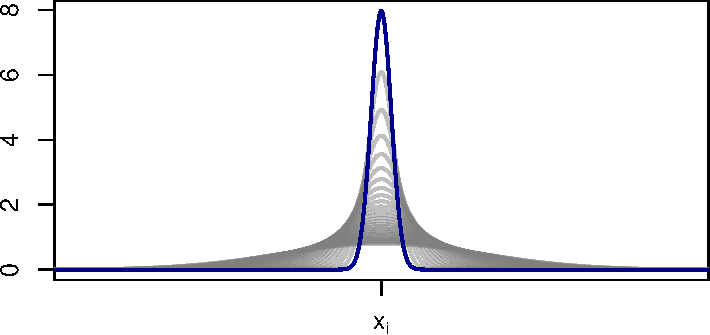
\includegraphics[width=0.9\linewidth]{Computational_Statistics_Script_files/figure-latex/dirac2-1} 

}

\caption{Normalverteilung mit $\mu_g=x_i$ für $\sigma_g\to 0$.}\label{fig:dirac2}
\end{figure}

😒 \textbf{Analytische Lösung:} Es ist zwar etwas mühsam, aber man kann versuchen die Log-Likelihood analytisch zu maximieren. Tut man sich das an, kommt man zu folgenden Ausdrücken:
\begin{align*}
\hat\pi_g&=\frac{1}{n}\sum_{i=1}^np_{ig}\\
\hat\mu_g&=\sum_{i=1}^n\frac{p_{ig}}{\left(\sum_{j=1}^np_{jg}\right)}x_i\\
\hat\sigma_g&=\sqrt{\sum_{i=1}^n\frac{p_{ig}}{\left(\sum_{j=1}^np_{jg}\right)}\left(x_i-\hat\mu_g\right)^2}
\end{align*}
für \(g=1,\dots,G\).

\begin{quote}
Die Herleitung der Ausdrücke für \(\hat{\mu}_g\), \(\hat{\sigma}_g\) und \(\hat{\pi}_g\) ist wirklich etwas lästig (mehrfache Anwendungen der Kettenregel, Produktregel, etc., sowie Anwendung des Lagrange-Multiplikator Verfahrens zur Optimierung unter Nebenbedingungen) aber machbar. In einer der Übungsaufgaben dürfen Sie den Ausdruck für \(\hat\mu_g\) herleiten.
\end{quote}

🙈 {\textbf{Aber:}} Diese Ausdrücke für \(\hat\pi_g\), \(\hat\mu_g\) und \(\hat\sigma_g\) hängen von den {\textbf{unbekannten}} Parametern \(\boldsymbol{\pi}=(\pi_1,\dots,\pi_G)\), \(\boldsymbol{\mu}=(\mu_1,\dots,\mu_G)\) und \(\boldsymbol{\sigma}=(\sigma_1,\dots,\sigma_G)\), denn:
\[
p_{ig}=\frac{\pi_gf(x_i|\mu_g,\sigma_g)}{f_G(x_i|\boldsymbol{\pi},\boldsymbol{\mu},\boldsymbol{\sigma})}
\]
für \(i=1,\dots,n\) und \(g=1,\dots,G\). Die Ausdrücke für \(\hat\pi_g\), \(\hat\mu_g\), und \(\hat\sigma_g\) erlauben also keine keine direkte Schätzung der unbekannten Parameter \(\pi_g\), \(\mu_g\) und \(\sigma_g\).

🥳 {\textbf{Lösung: Der EM Algorithmus}}

\hypertarget{ch:EM1}{%
\subsection{Der EM Algorithmus für GMMs}\label{ch:EM1}}

Die Ausdrücke für \(\hat\pi_g\), \(\hat\mu_g\) und \(\hat\sigma_g\) legen jedoch ein einfaches, iteratives ML-Schätzverfahren nahe: Nämlich einer alternierenden Schätzung von \(p_{ig}\) und \((\hat\pi_g, \hat\mu_g,\hat\sigma_g)\).

\textbf{Der Der EM Algorithmus:}

\begin{enumerate}
\def\labelenumi{\arabic{enumi}.}
\item
  Setze Startwerte \(\boldsymbol{\pi}^{(0)}\), \(\boldsymbol{\mu}^{(0)}\) und \(\boldsymbol{\sigma}^{(0)}\)
\item
  Für \(r=1,2,\dots\)

  \begin{itemize}
  \item
    {\textbf{(Expectation)}} Berechne:
    \[p_{ig}^{(r)}=\frac{\pi_g^{(r-1)}f(x_i|\mu^{(r-1)}_g,\sigma_g^{(r-1)})}{f_G(x_i|\boldsymbol{\pi}^{(r-1)},\boldsymbol{\mu}^{(r-1)},\boldsymbol{\sigma}^{(r-1)})}\]
  \item
    {\textbf{(Maximization)}} Berechne:

    \(\hat\pi_g^{(r)}=\frac{1}{n}\sum_{i=1}^np_{ig}^{(r)},\quad\quad\hat\mu_g^{(r)}=\sum_{i=1}^n\frac{p_{ig}^{(r)}}{\left(\sum_{j=1}^np_{jg}^{(r)}\right)}x_i\)

    \(\hat\sigma_g^{(r)}=\sqrt{\sum_{i=1}^n\frac{p_{ig}^{(r)}}{\left(\sum_{j=1}^np_{jg}^{(r)}\right)}\left(x_i-\hat\mu_g^{(r)}\right)^2}\)
  \end{itemize}
\item
  Prüfe Konvergenz:

  \begin{itemize}
  \tightlist
  \item
    Stoppe, falls sich der Wert der maximierten Log-Likelihood Funktion, \(\ell(\boldsymbol{\pi}^{(r)},\boldsymbol{\mu}^{(r)},\boldsymbol{\sigma}^{(r)}|\mathbf{z})\), nicht mehr ändert.
  \end{itemize}
\end{enumerate}

Der obige pseudo-Code wird im Folgenden Code-Chunck umgesetzt:

\begin{Shaded}
\begin{Highlighting}[]
\FunctionTok{library}\NormalTok{(}\StringTok{"MASS"}\NormalTok{)}
\FunctionTok{library}\NormalTok{(}\StringTok{"mclust"}\NormalTok{)}

\DocumentationTok{\#\# Daten:}
\NormalTok{x }\OtherTok{\textless{}{-}} \FunctionTok{cbind}\NormalTok{(Penguine\_Flosse) }\CommentTok{\# Daten [n x d]{-}Dimensional. }
\NormalTok{d }\OtherTok{\textless{}{-}} \FunctionTok{ncol}\NormalTok{(x)                }\CommentTok{\# Dimension (d=1: univariat)}
\NormalTok{n }\OtherTok{\textless{}{-}} \FunctionTok{nrow}\NormalTok{(x)                }\CommentTok{\# Stichprobenumfang}
\NormalTok{G }\OtherTok{\textless{}{-}} \DecValTok{2}                      \CommentTok{\# Anzahl Gruppen}

\DocumentationTok{\#\# Weitere Deklarationen:}
\NormalTok{llk       }\OtherTok{\textless{}{-}} \FunctionTok{matrix}\NormalTok{(}\ConstantTok{NA}\NormalTok{, n, G)}
\NormalTok{p         }\OtherTok{\textless{}{-}} \FunctionTok{matrix}\NormalTok{(}\ConstantTok{NA}\NormalTok{, n, G)  }
\NormalTok{loglikOld }\OtherTok{\textless{}{-}} \FloatTok{1e07}
\NormalTok{tol       }\OtherTok{\textless{}{-}} \FloatTok{1e{-}05}
\NormalTok{it        }\OtherTok{\textless{}{-}} \DecValTok{0}
\NormalTok{check     }\OtherTok{\textless{}{-}} \ConstantTok{TRUE} 


\DocumentationTok{\#\# EM Algorithmus}

\DocumentationTok{\#\# 1. Startwerte für pi, mu und sigma:}
\NormalTok{pi    }\OtherTok{\textless{}{-}} \FunctionTok{rep}\NormalTok{(}\DecValTok{1}\SpecialCharTok{/}\NormalTok{G, G)              }\CommentTok{\# Naive pi}
\NormalTok{sigma }\OtherTok{\textless{}{-}} \FunctionTok{array}\NormalTok{(}\FunctionTok{diag}\NormalTok{(d), }\FunctionTok{c}\NormalTok{(d,d,G)) }\CommentTok{\# Varianz = 1}
\NormalTok{mu    }\OtherTok{\textless{}{-}} \FunctionTok{t}\NormalTok{(MASS}\SpecialCharTok{::}\FunctionTok{mvrnorm}\NormalTok{(G, }\FunctionTok{colMeans}\NormalTok{(x), sigma[,,}\DecValTok{1}\NormalTok{]}\SpecialCharTok{*}\DecValTok{4}\NormalTok{) )}

\ControlFlowTok{while}\NormalTok{(check)\{}
  
  \DocumentationTok{\#\# 2.a Expectation{-}Schritt }
  \ControlFlowTok{for}\NormalTok{(g }\ControlFlowTok{in} \DecValTok{1}\SpecialCharTok{:}\NormalTok{G)\{}
\NormalTok{    p[,g] }\OtherTok{\textless{}{-}}\NormalTok{ pi[g] }\SpecialCharTok{*}\NormalTok{ mclust}\SpecialCharTok{:::}\FunctionTok{dmvnorm}\NormalTok{(x, mu[,g], sigma[,,g])}
\NormalTok{  \}}
\NormalTok{  p }\OtherTok{\textless{}{-}} \FunctionTok{sweep}\NormalTok{(p, }\DecValTok{1}\NormalTok{, }\AttributeTok{STATS =} \FunctionTok{rowSums}\NormalTok{(p), }\AttributeTok{FUN =} \StringTok{"/"}\NormalTok{)}
  
  \DocumentationTok{\#\# 2.b Maximization{-}Schritt}
\NormalTok{  par   }\OtherTok{\textless{}{-}}\NormalTok{ mclust}\SpecialCharTok{::}\FunctionTok{covw}\NormalTok{(x, p, }\AttributeTok{normalize =} \ConstantTok{FALSE}\NormalTok{)}
\NormalTok{  mu    }\OtherTok{\textless{}{-}}\NormalTok{ par}\SpecialCharTok{$}\NormalTok{mean}
\NormalTok{  sigma }\OtherTok{\textless{}{-}}\NormalTok{ par}\SpecialCharTok{$}\NormalTok{S}
\NormalTok{  pi    }\OtherTok{\textless{}{-}} \FunctionTok{colMeans}\NormalTok{(p)}
  
  \DocumentationTok{\#\# 3. Prüfung der Konvergenz}
  \ControlFlowTok{for}\NormalTok{(g }\ControlFlowTok{in} \DecValTok{1}\SpecialCharTok{:}\NormalTok{G) \{}
\NormalTok{    llk[,g] }\OtherTok{\textless{}{-}}\NormalTok{ pi[g] }\SpecialCharTok{*}\NormalTok{ mclust}\SpecialCharTok{:::}\FunctionTok{dmvnorm}\NormalTok{(x, mu[,g], sigma[,,g])}
\NormalTok{  \}}
\NormalTok{  loglik }\OtherTok{\textless{}{-}} \FunctionTok{sum}\NormalTok{(}\FunctionTok{log}\NormalTok{(}\FunctionTok{rowSums}\NormalTok{(llk))) }\CommentTok{\# aktueller max. Log{-}Likelihood Wert}
  \DocumentationTok{\#\#}
\NormalTok{  diff      }\OtherTok{\textless{}{-}} \FunctionTok{abs}\NormalTok{(loglik }\SpecialCharTok{{-}}\NormalTok{ loglikOld)}\SpecialCharTok{/}\FunctionTok{abs}\NormalTok{(loglik) }\CommentTok{\# Änderungsrate}
\NormalTok{  loglikOld }\OtherTok{\textless{}{-}}\NormalTok{ loglik}
\NormalTok{  it        }\OtherTok{\textless{}{-}}\NormalTok{ it }\SpecialCharTok{+} \DecValTok{1}
  \DocumentationTok{\#\# Änderungsrate noch groß genug (\textgreater{} tol)?}
\NormalTok{  check     }\OtherTok{\textless{}{-}}\NormalTok{ diff }\SpecialCharTok{\textgreater{}}\NormalTok{ tol}
\NormalTok{\}}

\DocumentationTok{\#\# Schätz{-}Resultate:}
\NormalTok{results }\OtherTok{\textless{}{-}} \FunctionTok{matrix}\NormalTok{(}\FunctionTok{c}\NormalTok{(pi, mu, }\FunctionTok{sqrt}\NormalTok{(sigma)), }
                  \AttributeTok{nrow =} \DecValTok{3}\NormalTok{, }\AttributeTok{ncol =} \DecValTok{2}\NormalTok{, }\AttributeTok{byrow =} \ConstantTok{TRUE}\NormalTok{,}
                  \AttributeTok{dimnames =} \FunctionTok{list}\NormalTok{(}
            \FunctionTok{c}\NormalTok{(}\StringTok{"Gewichte"}\NormalTok{, }\StringTok{"Mittelwerte"}\NormalTok{, }\StringTok{"Standardabweichungen"}\NormalTok{),}
            \FunctionTok{c}\NormalTok{(}\StringTok{"Gruppe 1"}\NormalTok{, }\StringTok{"Gruppe 2"}\NormalTok{))) }
\DocumentationTok{\#\#}
\NormalTok{results }\SpecialCharTok{\%\textgreater{}\%} \FunctionTok{round}\NormalTok{(., }\DecValTok{2}\NormalTok{)}
\CommentTok{\#\textgreater{}                      Gruppe 1 Gruppe 2}
\CommentTok{\#\textgreater{} Gewichte                 0.69     0.31}
\CommentTok{\#\textgreater{} Mittelwerte            216.20   194.26}
\CommentTok{\#\textgreater{} Standardabweichungen     7.32     6.27}
\end{Highlighting}
\end{Shaded}

\textbf{Das Clusterverfahren basierend auf Gaußschen Mischverteilungen:}

\begin{enumerate}
\def\labelenumi{\arabic{enumi}.}
\tightlist
\item
  Gaußsche Mischverteilung (\textbf{per EM Algorithmus}) schätzen
\item
  Die Datenpunkte \(x_i\) derjenigen Gruppe \(g\) zuordnen, welche die \textbf{a-posteriori-Wahrscheinlichkeit} \(p_{ig}\) maximiert.
\end{enumerate}

Das finale Schätzergebnis erlaubt es uns, Abbildung \ref{fig:GMM-plot1} zu replizieren.

\begin{Shaded}
\begin{Highlighting}[]
\DocumentationTok{\#\# Auswerten der Gaußsche Mischungs{-}Dichtefunktion}
\NormalTok{np      }\OtherTok{\textless{}{-}} \DecValTok{100} \CommentTok{\# Anzahl der Auswertungspunkte}
\NormalTok{xxd     }\OtherTok{\textless{}{-}} \FunctionTok{seq}\NormalTok{(}\FunctionTok{min}\NormalTok{(Penguine\_Flosse)}\SpecialCharTok{{-}}\DecValTok{3}\NormalTok{, }\FunctionTok{max}\NormalTok{(Penguine\_Flosse)}\SpecialCharTok{+}\DecValTok{5}\NormalTok{, }\AttributeTok{length.out =}\NormalTok{ np)}
\DocumentationTok{\#\# Mischungs{-}Dichte}
\NormalTok{yyd     }\OtherTok{\textless{}{-}} \FunctionTok{dnorm}\NormalTok{(xxd, mu[}\DecValTok{1}\NormalTok{,}\DecValTok{1}\NormalTok{], }\FunctionTok{sqrt}\NormalTok{(sigma)[,,}\DecValTok{1}\NormalTok{])}\SpecialCharTok{*}\NormalTok{pi[}\DecValTok{1}\NormalTok{] }\SpecialCharTok{+}
           \FunctionTok{dnorm}\NormalTok{(xxd, mu[}\DecValTok{1}\NormalTok{,}\DecValTok{2}\NormalTok{], }\FunctionTok{sqrt}\NormalTok{(sigma)[,,}\DecValTok{2}\NormalTok{])}\SpecialCharTok{*}\NormalTok{pi[}\DecValTok{2}\NormalTok{]}
\DocumentationTok{\#\# Einzel{-}Dichten}
\NormalTok{yyd1    }\OtherTok{\textless{}{-}} \FunctionTok{dnorm}\NormalTok{(xxd, mu[}\DecValTok{1}\NormalTok{,}\DecValTok{1}\NormalTok{], }\FunctionTok{sqrt}\NormalTok{(sigma)[,,}\DecValTok{1}\NormalTok{])}\SpecialCharTok{*}\NormalTok{pi[}\DecValTok{1}\NormalTok{]}
\NormalTok{yyd2    }\OtherTok{\textless{}{-}} \FunctionTok{dnorm}\NormalTok{(xxd, mu[}\DecValTok{1}\NormalTok{,}\DecValTok{2}\NormalTok{], }\FunctionTok{sqrt}\NormalTok{(sigma)[,,}\DecValTok{2}\NormalTok{])}\SpecialCharTok{*}\NormalTok{pi[}\DecValTok{2}\NormalTok{]}

\DocumentationTok{\#\# Plot}
\FunctionTok{hist}\NormalTok{(}\AttributeTok{x =}\NormalTok{ Penguine\_Flosse, }\AttributeTok{xlab=}\StringTok{"Flossenlänge (mm)"}\NormalTok{, }\AttributeTok{main=}\StringTok{"Pinguine}\SpecialCharTok{\textbackslash{}n}\StringTok{(Zwei Gruppen)"}\NormalTok{,}
     \AttributeTok{col=}\FunctionTok{gray}\NormalTok{(.}\DecValTok{65}\NormalTok{,.}\DecValTok{5}\NormalTok{), }\AttributeTok{border=}\FunctionTok{gray}\NormalTok{(.}\DecValTok{35}\NormalTok{,.}\DecValTok{5}\NormalTok{), }\AttributeTok{freq =} \ConstantTok{FALSE}\NormalTok{, }\AttributeTok{ylim=}\FunctionTok{c}\NormalTok{(}\DecValTok{0}\NormalTok{, }\FloatTok{0.04}\NormalTok{))}
\FunctionTok{lines}\NormalTok{(}\AttributeTok{x =}\NormalTok{ xxd, }\AttributeTok{y=}\NormalTok{yyd, }\AttributeTok{lwd=}\DecValTok{2}\NormalTok{, }\AttributeTok{col=}\FunctionTok{gray}\NormalTok{(.}\DecValTok{35}\NormalTok{,.}\DecValTok{75}\NormalTok{))}
\FunctionTok{lines}\NormalTok{(}\AttributeTok{x =}\NormalTok{ xxd, }\AttributeTok{y=}\NormalTok{yyd1, }\AttributeTok{lwd=}\DecValTok{2}\NormalTok{, }\AttributeTok{col=}\FunctionTok{gray}\NormalTok{(.}\DecValTok{35}\NormalTok{,.}\DecValTok{75}\NormalTok{), }\AttributeTok{lty=}\DecValTok{2}\NormalTok{)}
\FunctionTok{lines}\NormalTok{(}\AttributeTok{x =}\NormalTok{ xxd, }\AttributeTok{y=}\NormalTok{yyd2, }\AttributeTok{lwd=}\DecValTok{2}\NormalTok{, }\AttributeTok{col=}\FunctionTok{gray}\NormalTok{(.}\DecValTok{35}\NormalTok{,.}\DecValTok{75}\NormalTok{), }\AttributeTok{lty=}\DecValTok{2}\NormalTok{)}
\FunctionTok{abline}\NormalTok{(}\AttributeTok{v=}\FloatTok{203.1}\NormalTok{, }\AttributeTok{lty=}\DecValTok{3}\NormalTok{)}
\FunctionTok{stripchart}\NormalTok{(Penguine\_Flosse[class}\SpecialCharTok{==}\DecValTok{1}\NormalTok{], }\AttributeTok{method =} \StringTok{"jitter"}\NormalTok{, }\AttributeTok{jitter =}\NormalTok{ .}\DecValTok{0005}\NormalTok{, }\AttributeTok{at =}\NormalTok{ .}\DecValTok{001}\NormalTok{,}
           \AttributeTok{pch =} \DecValTok{21}\NormalTok{, }\AttributeTok{col=}\FunctionTok{alpha}\NormalTok{(col\_v[}\DecValTok{1}\NormalTok{],.}\DecValTok{5}\NormalTok{), }\AttributeTok{bg=}\FunctionTok{alpha}\NormalTok{(col\_v[}\DecValTok{1}\NormalTok{],.}\DecValTok{5}\NormalTok{), }\AttributeTok{cex=}\FloatTok{1.3}\NormalTok{, }\AttributeTok{add =} \ConstantTok{TRUE}\NormalTok{)}
\FunctionTok{stripchart}\NormalTok{(Penguine\_Flosse[class}\SpecialCharTok{==}\DecValTok{2}\NormalTok{], }\AttributeTok{method =} \StringTok{"jitter"}\NormalTok{, }\AttributeTok{jitter =}\NormalTok{ .}\DecValTok{0005}\NormalTok{, }\AttributeTok{at =}\NormalTok{ .}\DecValTok{001}\NormalTok{,}
           \AttributeTok{pch =} \DecValTok{21}\NormalTok{, }\AttributeTok{col=}\FunctionTok{alpha}\NormalTok{(col\_v[}\DecValTok{2}\NormalTok{],.}\DecValTok{5}\NormalTok{), }\AttributeTok{bg=}\FunctionTok{alpha}\NormalTok{(col\_v[}\DecValTok{2}\NormalTok{],.}\DecValTok{5}\NormalTok{), }\AttributeTok{cex=}\FloatTok{1.3}\NormalTok{, }\AttributeTok{add =} \ConstantTok{TRUE}\NormalTok{)}
\end{Highlighting}
\end{Shaded}

\begin{center}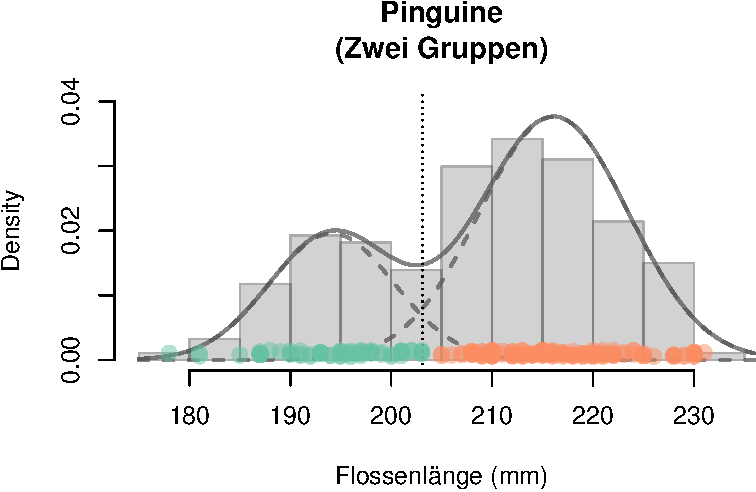
\includegraphics[width=0.9\linewidth]{Computational_Statistics_Script_files/figure-latex/unnamed-chunk-13-1} \end{center}

\hypertarget{der-alternative-wahre-blick-auf-den-em-algorithmus}{%
\section{Der alternative (wahre) Blick auf den EM Algorithmus}\label{der-alternative-wahre-blick-auf-den-em-algorithmus}}

Der EM Algorithmus ermöglicht es Maximum Likelihood Probleme zu vereinfachen, indem man die Daten durch nicht beobachtete („latente``) Variablen vervollständigt. Dieses Prinzip ist der eigentliche wahre Beitrag des EM Algorithmus. Es ermöglicht die Lösung verschiedener Maximum Likelihood Probleme - wir bleiben aber hier bei der Schätzung von GMMs.

\begin{quote}
\textbf{Zur Erinnerung:} Wir haben es ja nicht geschafft, die Log-Likelihood Funktion
\[
\ell(\boldsymbol{\pi},\boldsymbol{\mu},\boldsymbol{\sigma}|\mathbf{x})
=\sum_{i=1}^n\ln\left(\sum_{g=1}^G\pi_gf(x_i|\mu_g,\sigma_g)\right)
\]
direkt zu maximieren. Die \(\ln(\sum_{g=1}^G[\dots])\)-Konstruktion macht einem hier das Leben schwer.
\end{quote}

\hypertarget{vervollstuxe4ndigung-der-daten}{%
\subsection{Vervollständigung der Daten}\label{vervollstuxe4ndigung-der-daten}}

In unseren Pinguin-Daten gibt zwei Gruppen (\(g\in\{1,2\}\)). Es gäbe also im Prinzip \(G=2\)-dimensionale Zuordnungsvektoren \((z_{i1},z_{i2})\) mit
\[
(z_{i1},z_{i2})=
\left\{\begin{array}{ll}
(1,0)&\text{falls Pinguin }i\text{ zu Gruppe }g=1\text{ gehört.}\\
(0,1)&\text{falls Pinguin }i\text{ zu Gruppe }g=2\text{ gehört.}\\
\end{array}\right.
\]
Im Fall von \(G>2\) Gruppen:\\
\[
(z_{i1},\dots,z_{ig},\dots,z_{iG})=
\left\{\begin{array}{ll}
(1,0,\dots,0)&\text{falls Datenpunkt }i\text{ zu Gruppe }g=1\text{ gehört.}\\
(0,1,\dots,0)&\text{falls Datenpunkt }i\text{ zu Gruppe }g=2\text{ gehört.}\\
\quad\quad\vdots&\\
(0,0,\dots,1)&\text{falls Datenpunkt }i\text{ zu Gruppe }g=G\text{ gehört.}\\
\end{array}\right.
\]

Die Zuordnungen \(z_{ig}\) können also die Werte \(z_{ig}\in\{0,1\}\) annehmen, wobei aber gelten muss, dass \(\sum_{g=1}^Gz_{ig}=1\).

\begin{quote}
\textbf{Beachte:} Für jeden Datenpunkt \(i\) (jeder Pinguin \(i\)) gibt es nur \textbf{eine} Gruppe (daher \(\sum_{g=1}^Gz_{ig}=1\)). Dies ist eine wichtige Restriktion von GMMs, welche bei den Pinguindaten unproblematisch ist. Bei Anwendungen mit hirarchischen Gruppierungen ist dies aber evtl. problematisch.
\end{quote}

Die Zuordnungen \(z_{ig}\) sind leider unbekannt (latent). Wir wissen aber trotzdem etwas über diese Zuordnungen. Die Gewichte \(\pi_1,\dots,\pi_G\) der Gaußschen Mischverteilung
\[
f_G(x|\boldsymbol{\pi},\boldsymbol{\mu},\boldsymbol{\sigma})=\sum_{g=1}^G\pi_gf(x|\mu_g,\sigma_g),
\]
geben die Anteile der Einzelverteilungen \(f(\cdot|\mu_g,\sigma_g)\) an der Gesamtverteilung \(f_G\) an. Im Schnitt kommen also \(\pi_g\cdot 100\%\) der Datenpunkte von Gruppe \(g\), \(g=1,\dots,G\). Somit können wir die (latente) Zuordnung \(z_{ig}\) als eine Realisation der Zufallsvariablen \(Z_{ig}\) mit Wahrscheinlichkeitsfunktion
\[
P(Z_{ig}=1)=\pi_g
\]
auffassen.

Wegen der Bedingung \(\sum_{g=1}^Gz_{ig}=1\), gilt dass
\[
Z_{ig}=1\quad \Rightarrow\quad Z_{i1}=0,\dots,Z_{ig-1}=0,Z_{ig+1}=0,\dots,Z_{iG}=0.
\]

\hypertarget{a-priori-und-a-posteriori-wahrscheinlichkeiten-pi_g-und-p_ig}{%
\subsection{\texorpdfstring{A-priori und A-posteriori Wahrscheinlichkeiten: \(\pi_g\) und \(p_{ig}\)}{A-priori und A-posteriori Wahrscheinlichkeiten: \textbackslash pi\_g und p\_\{ig\}}}\label{a-priori-und-a-posteriori-wahrscheinlichkeiten-pi_g-und-p_ig}}

\textbf{A-priori-Wahrscheinlichkeit \(\pi_g\):} Man bezeichnet die Wahrscheinlichkeiten \(\pi_g\) als die \emph{a-priori-Wahrscheinlichkeiten}. Wenn wir nichts über die Flossenlänge von Pinguin \(i\) wissen, dann bleiben uns nur die a-priori-Wahrscheinlichkeiten:

„Mit Wahrscheinlichkeit \(\pi_g=P(Z_{ig}=1)\) gehört Pinguin \(i\) zu Gruppe \(g\).``

\textbf{A-posteriori-Wahrscheinlichkeit \(\;p_{ig}\):} Falls wir die Flossenlänge \(x_i\) von Pinguin \(i\) erfahren, können wir die a-priori-Wahrscheinlichkeiten mit Hilfe des \textbf{Satzes von Bayes} aktualisieren. Dies führt dann zur \emph{a-posteriori-Wahrscheinlichkeit}:

„Mit Wahrscheinlichkeit \(p_{ig}=P(Z_{ig=1}|X_i=x_i)\) gehört ein Pinguin \(i\) mit Flossenlänge \(x_i\) zu Gruppe \(g\).

\textbf{Satz von Bayes:}
\begin{align*}
p_{ig}
&=\frac{\pi_gf(x_i|\mu_g,\sigma_g)}{f_G(x_i|\boldsymbol{\pi},\boldsymbol{\mu},\boldsymbol{\sigma})}\\[2ex]
&=\frac{\overbrace{P(Z_{ig}=1)}^{\text{„A-priori-Wahrs.“}}f(x_i|\mu_g,\sigma_g)}{f_G(x_i|\boldsymbol{\pi},\boldsymbol{\mu},\boldsymbol{\sigma})}=\overbrace{P(Z_{ig}=1|X_i=x_i)}^{\text{„A-posteriori-Wahrs.“}}=p_{ig}\\
\end{align*}

\hypertarget{der-bedingte-mittelwert-p_ig}{%
\subsection{\texorpdfstring{Der (bedingte) Mittelwert: \(p_{ig}\)}{Der (bedingte) Mittelwert: p\_\{ig\}}}\label{der-bedingte-mittelwert-p_ig}}

\textbf{Beachte:} Die a-posteriori-Wahrscheinlichkeiten \(p_{ig}\) sind tatsächlich (bedingte) Erwartungswerte:
\begin{align*}
p_{ig}&= 1\cdot P(Z_{ig}=1|X_i=x_i)+0\cdot P(Z_{ig}=0|X_i=x_i) = E(Z_{ig}|X_i=x_i)\\
\end{align*}
Damit ist die Berechnung von \(p_{ig}\) im \textbf{(Expectation)}-Schritt des EM Algorithmuses (siehe Kapitel \ref{ch:EM1}) also tatsächlich eine Erwartungswertberechnung.

\hypertarget{das-grouxdfe-ganze}{%
\section{Das Große Ganze}\label{das-grouxdfe-ganze}}

Hätten wir neben den Datenpunkten \(\mathbf{x}=(x_1,\dots,x_n)\) auch die Gruppenzuordnungen \(\mathbf{z}=(z_{11},\dots,z_{nG})\) beobachtet, dann könnten wir folgende \textbf{Likelihood (\(\tilde{\mathcal{L}}\)) bzw. Log-Likelihood (\(\tilde{\ell}\)) Funktion} aufstellen:
\begin{align*}
\tilde{\mathcal{L}}(\boldsymbol{\pi},\boldsymbol{\mu},\boldsymbol{\sigma}|\mathbf{x},\mathbf{z})
&=\prod_{i=1}^n\prod_{g=1}^G\left(\pi_gf(x_i|\mu_g,\sigma_g)\right)^{z_{ig}}\\[2ex]
\tilde{\ell}(\boldsymbol{\pi},\boldsymbol{\mu},\boldsymbol{\sigma}|\mathbf{x},\mathbf{z})
&=\sum_{i=1}^n\sum_{g=1}^Gz_{ig}\left\{\ln\left(\pi_g\right)+\ln\left(f(x_i|\mu_g,\sigma_g)\right)\right\}
\end{align*}

\begin{itemize}
\item
  Im Gegensatz zur ursprünglichen Log-Likelihood Funktion (\(\ell\)), wäre die neue Log-Likelihood Funktion \(\tilde\ell\) \textbf{einfach zu maximieren}, da hier keine Summe innerhalb der Logarithmusfunktion steckt, sodass wir direkt den Logarithmus der Normalverteilung berechnen können. Dies vereinfacht das Maximierungsproblem deutlich, da die Normalverteilung zur Exponentialfamilie gehört.
\item
  Aber: Wir beobachten die Realisationen \(\mathbf{z}=(z_{11},\dots,z_{nG})\) nicht, sondern kennen lediglich die Verteilung der Zufallsvariablen \(\mathbf{Z}=(Z_{11},\dots,Z_{nG})\). Dies führt zu einer stochastischen Version der Log-Likelihood Funktion:
  \[
  \tilde{\ell}(\boldsymbol{\pi},\boldsymbol{\mu},\boldsymbol{\sigma}|\mathbf{x},\mathbf{Z})=\sum_{i=1}^n\sum_{g=1}^GZ_{ig}\left\{\ln\left(\pi_g\right)+\ln\left(f(x_i|\mu_g,\sigma_g)\right)\right\}
  \]
\item
  Von dieser können jedoch den bedingten Erwartungswert berechnen:
  \[
  E(\tilde{\ell}(\boldsymbol{\pi},\boldsymbol{\mu},\boldsymbol{\sigma}|\mathbf{x},\mathbf{z})|X_i=x_i)=\sum_{i=1}^n\sum_{g=1}^Gp_{ig}\left\{\ln\left(\pi_g\right)+\ln\left(f(x_i|\mu_g,\sigma_g)\right)\right\}
  \]
\end{itemize}

\hypertarget{ch:EM2}{%
\subsection{\texorpdfstring{Der EM Algorithmus: \emph{Die abstrakte Version}}{Der EM Algorithmus: Die abstrakte Version}}\label{ch:EM2}}

Der folgende EM Algorithmus unterscheidet sich wieder lediglich in der Notation von den oben bereits besprochenen Versionen (siehe Kapitel \ref{ch:EM1}). Die hier gewählte Notation verdeutlicht, dass der \textbf{Expectation}-Schritt die zu maximierende Log-Likelihood Funktion aktualisiert und diese dann im \textbf{(Maximization)}-Schritt maximiert wird. Darüber hinaus ist die gewählte Notation abstrakt genug, um die Grundidee des EM Algorithmuses auf andere Maximum Likelihood Probleme zu übertragen. Im Folgenden wird der Parametervektor \((\boldsymbol{\pi},\boldsymbol{\mu},\boldsymbol{\sigma})\) der Einfachheit halber auch mit \(\boldsymbol{\theta}\) bezeichnet.

\begin{enumerate}
\def\labelenumi{\arabic{enumi}.}
\item
  Setze Startwerte \(\boldsymbol{\theta}^{(0)}=(\pi^{(0)}, \mu^{(0)}, \sigma^{(0)})\)
\item
  Für \(r=1,2,\dots\)

  \begin{itemize}
  \item
    {\textbf{(Expectation)} } Berechne:
    \begin{align*}
     \mathcal{Q}(\boldsymbol{\theta},\boldsymbol{\theta}^{(r-1)})
     &=E_{\boldsymbol{\theta}^{(r-1)}}(\tilde{\ell}(\boldsymbol{\pi},\boldsymbol{\mu},\boldsymbol{\sigma}|\mathbf{x},\mathbf{z})|X_i=x_i)\\
     &=\sum_{i=1}^n\sum_{k=1}^Kp_{ig}^{(r-1)}\left\{\ln\left(\pi_g\right)+\ln\left(f(x_i|\mu_g,\sigma_g)\right)\right\}
     \end{align*}
  \item
    {\textbf{(Maximization)}} Berechne:
    \begin{align*}
     \boldsymbol{\theta}^{(r)}=\arg\max_{\boldsymbol{\theta}}\mathcal{Q}(\boldsymbol{\theta},\boldsymbol{\theta}^{(r-1)})
     \end{align*}
  \end{itemize}
\item
  Prüfe Konvergenz:

  \begin{itemize}
  \tightlist
  \item
    Stoppe, falls sich der Wert der maximierten Log-Likelihood Funktion, \(\mathcal{Q}(\boldsymbol{\theta}^{(r)},\boldsymbol{\theta}^{(r-1)})\), nicht mehr ändert.
  \end{itemize}
\end{enumerate}

\hypertarget{ende}{%
\subsection*{Ende}\label{ende}}
\addcontentsline{toc}{subsection}{Ende}

Dem gemeinen Pinguin ist der EM Algorithmus egal.

\hypertarget{ch:RegML}{%
\chapter{Regressionsmodelle im Kontext des Maschinellen Lernens}\label{ch:RegML}}

\textbf{Lineare Regressionsmodelle} gehören zu den erfolgreichsten statistischen Modellen, da sie

\begin{itemize}
\tightlist
\item
  vergleichsweise \textbf{einfach zu interpretieren} sind und
\item
  zugleich \textbf{äußerst flexibel} sind.
\end{itemize}

In diesem Kapitel betrachten wir das multivariate (oder multiple) lineare Regressionsmodell als \textbf{Prädiktionsmodell} im Kontext des maschinellen Lernens.

\hypertarget{lernziele-fuxfcr-dieses-kapitel-1}{%
\subsection*{Lernziele für dieses Kapitel}\label{lernziele-fuxfcr-dieses-kapitel-1}}
\addcontentsline{toc}{subsection}{Lernziele für dieses Kapitel}

Sie können \ldots{}

\begin{itemize}
\tightlist
\item
  ein \textbf{Anwendungsfeld} des linearen Regressionsmodell als Prädiktionsmodell \textbf{benennen}.
\item
  die \textbf{Probleme} der Auswahl eines geeigneten Prädiktionsmodells am Beispiel der Polynomregression \textbf{benennen und erläutern}.
\item
  die \textbf{Grundidee} der Validierungsdaten-Methode \textbf{erläutern}.
\item
  die \textbf{Grundidee} der k-fachen Kreuzvalidierung \textbf{erläutern}.
\end{itemize}

\hypertarget{begleitlektuxfcren-1}{%
\subsection*{Begleitlektüren}\label{begleitlektuxfcren-1}}
\addcontentsline{toc}{subsection}{Begleitlektüren}

Zur Vorbereitung der Klausur ist es grundsätzlich ausreichend dieses Kapitel durchzuarbeiten - aber Lesen hat ja noch nie geschadet. Empfehlenswerte weiterführende Literatur:

\begin{itemize}
\item
  Kapitel 3 in \href{https://trevorhastie.github.io/ISLR/}{\textbf{An Introduction to Statistical Learning, with Applications in R}} \citep{ISLR2021}.
  Die pdf-Version des Buches ist hier frei erhältlichen:
  \href{https://www.statlearning.com/}{\textbf{www.statlearning.com}}
\item
  Kapitel 3 in \href{https://www.microsoft.com/en-us/research/uploads/prod/2006/01/Bishop-Pattern-Recognition-and-Machine-Learning-2006.pdf}{\textbf{Pattern Recognition and Machine Learning}} \citep{book_Bishop2006}.
  Die pdf-Version des Buches ist frei erhältlichen: \href{https://www.microsoft.com/en-us/research/uploads/prod/2006/01/Bishop-Pattern-Recognition-and-Machine-Learning-2006.pdf}{\textbf{pdf-Version}}
\item
  Kapitel 6 in \href{https://www.econometrics-with-r.org/}{\textbf{Introduction to Econometrics with R}} \citep{IntroEconometricsR2021}.
  Freies Online-Buch: \href{https://www.econometrics-with-r.org/}{\textbf{www.econometrics-with-r.org}}
\end{itemize}

\hypertarget{r-pakete-und-datenbeispiel-fuxfcr-dieses-kapitel}{%
\subsection*{R-Pakete und Datenbeispiel für dieses Kapitel}\label{r-pakete-und-datenbeispiel-fuxfcr-dieses-kapitel}}
\addcontentsline{toc}{subsection}{R-Pakete und Datenbeispiel für dieses Kapitel}

Folgende Pakete werden in diesem Kapitel benötigt.

\begin{itemize}
\tightlist
\item
  \textbf{tidyverse}: Viele nützliche Pakete zur Datenverarbeitung.
\item
  \textbf{GGally}: Enthält die Funktion \texttt{ggpairs()} zur Erzeugung von Pairs-Plots
\item
  \textbf{ISLR}: Enthält die \texttt{Auto} Daten
\end{itemize}

Falls noch nicht geschehen, müssen diese Pakete installiert und geladen werden:

\begin{Shaded}
\begin{Highlighting}[]
\DocumentationTok{\#\# Installieren}
\FunctionTok{install.packages}\NormalTok{(}\StringTok{"tidyverse"}\NormalTok{) }
\FunctionTok{install.packages}\NormalTok{(}\StringTok{"GGally"}\NormalTok{)    }
\FunctionTok{install.packages}\NormalTok{(}\StringTok{"ISLR"}\NormalTok{)      }
\DocumentationTok{\#\# Laden}
\FunctionTok{library}\NormalTok{(}\StringTok{"tidyverse"}\NormalTok{) }\CommentTok{\# Viele nützliche Pakete zur Datenverarbeitung}
\FunctionTok{library}\NormalTok{(}\StringTok{"GGally"}\NormalTok{)    }\CommentTok{\# Pairs{-}Plot}
\FunctionTok{library}\NormalTok{(}\StringTok{"ISLR"}\NormalTok{)      }\CommentTok{\# Enthält die Auto{-}Daten}
\FunctionTok{data}\NormalTok{(Auto)           }\CommentTok{\# Auto{-}Daten abrufbar machen}
\end{Highlighting}
\end{Shaded}

Als Datenbeispiel für diese Kapitel betrachten wir den \texttt{Auto} Datensatz im R-Paket ISLR. Wir betrachten folgende Auswahl der Variablen im Datensatz \texttt{Auto}:

\begin{itemize}
\tightlist
\item
  \textbf{Zielvariable:}

  \begin{itemize}
  \tightlist
  \item
    \textbf{Verbrauch (km/Liter)}
  \end{itemize}
\item
  \textbf{Prädiktorvariablen:}

  \begin{itemize}
  \tightlist
  \item
    \textbf{Gewicht (kg):} Schwerere Autos verbrauchen wahrscheinlich mehr.
  \item
    \textbf{Leistung (PS):} Höhere Leistung geht wohl auch mit höherem Verbrauch einher.
  \item
    \textbf{Hubraum (ccm):} Großer Hubraum \ldots{} höherer Verbrauch?
  \end{itemize}
\end{itemize}

\textbf{Achtung:} Es gibt sicherlich noch weitere relevante Prädiktorvariablen. Obige Auswahl ist jedoch relativ einfach zu erheben und ermöglicht eventuell bereits eine \textbf{gute Prädiktion des Verbrauches} im Rahmen eines \textbf{Regressionsmodells}. Falls dem so ist, könnte unser Prädiktionsmodell dazu dienen, nach Auffälligkeiten bei den herstellerseitigen Verbrauchsangaben zu suchen. Besonders große Abweichung zwischen Modellprädiktion und Herstellerangabe wäre ein mögliches Indiz auf unlautere Zahlenschönung.

\textbf{Aufbereitung der Daten:}

\begin{Shaded}
\begin{Highlighting}[]
\DocumentationTok{\#\# Auswahl und Aufbereitung der Variablen }
\NormalTok{Auto\_df }\OtherTok{\textless{}{-}}\NormalTok{ Auto }\SpecialCharTok{\%\textgreater{}\%} 
  \FunctionTok{mutate}\NormalTok{(}\AttributeTok{Verbrauch =}\NormalTok{ mpg }\SpecialCharTok{*}\NormalTok{ (}\FloatTok{1.60934}\SpecialCharTok{/}\FloatTok{3.78541}\NormalTok{), }\CommentTok{\# Verbrauch (km/Liter)}
         \AttributeTok{Gewicht   =}\NormalTok{ weight }\SpecialCharTok{*} \FloatTok{0.45359}\NormalTok{,        }\CommentTok{\# Gewicht (kg)}
         \AttributeTok{PS        =}\NormalTok{ horsepower,              }\CommentTok{\# Pferdestärken (PS)}
         \AttributeTok{Hubraum   =}\NormalTok{ displacement }\SpecialCharTok{*} \FloatTok{2.54}\SpecialCharTok{\^{}}\DecValTok{3}    \CommentTok{\# Hubraum (ccm)}
\NormalTok{         ) }\SpecialCharTok{\%\textgreater{}\%}   
\NormalTok{ dplyr}\SpecialCharTok{::}\FunctionTok{select}\NormalTok{(}\StringTok{"Verbrauch"}\NormalTok{, }\StringTok{"Gewicht"}\NormalTok{, }\StringTok{"PS"}\NormalTok{, }\StringTok{"Hubraum"}\NormalTok{) }

\NormalTok{n }\OtherTok{\textless{}{-}} \FunctionTok{nrow}\NormalTok{(Auto\_df) }\CommentTok{\# Stichprobenumfang }
\end{Highlighting}
\end{Shaded}

Insgesamt enthält der betrachtete Datensatz also fünf Variablen zu \(n=392\) verschiedenen Autos. Dies sind die ersten sechs Zeilen des Datensatzes:

Verbrauch (km/Liter)

Gewicht (kg)

Pferdestärken (PS)

Hubraum (ccm)

7.65

1589.38

130

5030.83

6.38

1675.11

165

5735.47

7.65

1558.54

150

5211.09

6.80

1557.17

150

4981.67

7.23

1564.43

140

4948.89

6.38

1969.03

198

7030.05

Um sich einen Überblick zu den Beziehungen zwischen den Variablen zu verschaffen, eignet sich ein \textbf{Pairs-Plot} sehr gut (siehe Abbildung \ref{fig:pairsplot}):

\begin{Shaded}
\begin{Highlighting}[]
\FunctionTok{ggpairs}\NormalTok{(Auto\_df,}
\AttributeTok{upper =} \FunctionTok{list}\NormalTok{(}\AttributeTok{continuous =} \StringTok{"density"}\NormalTok{, }\AttributeTok{combo =} \StringTok{"box\_no\_facet"}\NormalTok{),}
\AttributeTok{lower =} \FunctionTok{list}\NormalTok{(}\AttributeTok{continuous =} \StringTok{"points"}\NormalTok{, }\AttributeTok{combo =} \StringTok{"dot\_no\_facet"}\NormalTok{))}
\end{Highlighting}
\end{Shaded}

\begin{figure}[h]

{\centering 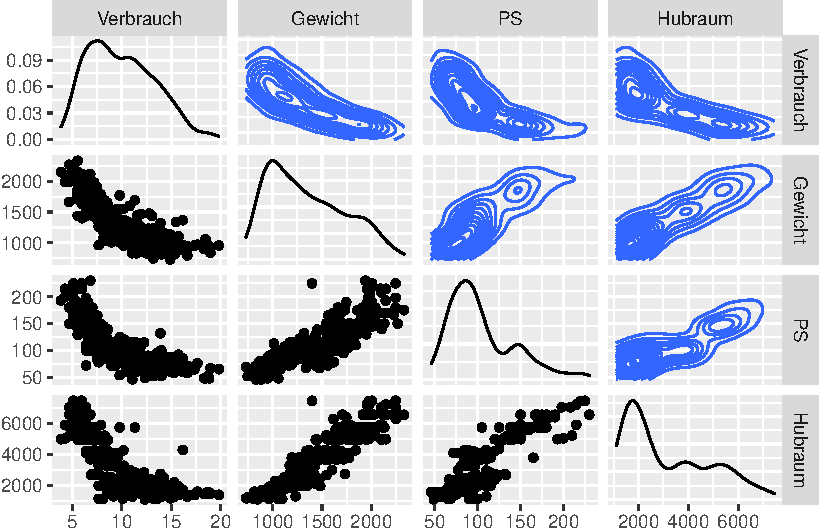
\includegraphics[width=1\linewidth,height=1\textheight]{Computational_Statistics_Script_files/figure-latex/pairsplot-1} 

}

\caption{Pairs-Plot zur Veranschaulichung der paarweisen Zusammenhänge zwischen den Variablen.}\label{fig:pairsplot}
\end{figure}

Der Pairs-Plot veranschaulicht alle paarweisen Zusammenhänge zwischen den Variablen im Datensatz \texttt{Auto\_df}. Uns interessieren hierbei in erster Linie die Zusammenhänge zwischen der Zielvariable \textbf{Verbrauch} und den \textbf{Prädiktorvariablen}:

\begin{itemize}
\tightlist
\item
  \(Y=\)\textbf{Verbrauch} und \ldots{}

  \begin{itemize}
  \tightlist
  \item
    \(G=\) \textbf{Gewicht}\(_i\)\textbf{:} haben einen nicht linearen, negativen Zusammenhang.
  \item
    \(P=\) \textbf{PS:} haben einen nicht linearen, negativen Zusammenhang.
  \item
    \(H=\) \textbf{Hubraum:} haben einen nicht linearen, negativen Zusammenhang.
  \end{itemize}
\end{itemize}

\hypertarget{das-allgemeine-regressionsmodell}{%
\section{Das allgemeine Regressionsmodell}\label{das-allgemeine-regressionsmodell}}

Die einzelnen Prädiktorvariablen werden gerne kompakt zu einer multivariaten Prädiktorvariablen \(X=(X_1,X_2,\dots,X_p)\) zusammengefasst; in unserem Benzinverbrauchsbeispiel also \(X=(G,P,H,B)\). So lässt sich das \textbf{allgemeines Regressionsmodell} schreiben als
\[
Y=f(X)+\varepsilon
\]
wobei

\begin{itemize}
\tightlist
\item
  \(f\) den \textbf{systematischen Zusammenhang} zwischen der Zielvariable \(Y\) und den Prädiktorvariablen \(X\) beschreibt und
\item
  \(\varepsilon\) ein \textbf{Fehlerterm} ist, der unabhängig von \(X\) ist und Mittelwert \(E(\varepsilon)=0\) Null hat.
\end{itemize}

Daraus ergibt sich folgender Zusammenhang zwischen der \textbf{allgemeinen Regressionsfunktion} \(f\) und dem bedingten Mittelwert von \(Y\) gegeben \(X\):
\[
E(Y|X)=f(X)
\]
Die Funktion \(f\) beschreibt also den bedingten Mittelwert von \(Y\) gegeben \(X\). Ziel ist es nun, die Regressionsfunktion \(f\) aus den Daten zu schätzen (lernen).

\textbf{Achtung:} Die Annahme der Unabhängigkeit zwischen \(\varepsilon\) und \(X\) kann in der Praxis verletzt sein. Die Verletzung dieser Unabhängigkeitsannahme erlaubt insbesondere keine kausale Interpretation der Ergebnisse, daher betrachtet die Literatur zur Kausalinferenz viele Möglichkeiten diese Unabhängigkeitsannahme durch eine weniger strikte Annahmen zu ersetzen. In der Literatur zur prädiktiven Inferenzen wird eine Verletzung der Unabhängigkeitsannahme weniger kritisch gesehen, da eine Prädiktion trotz verletzter Unabhängigkeitsannahme sehr gut sein kann. Eine schöne und gut lesbare Übersicht zu den Unterschieden zwischen der Kausalinferenz und der prädiktiven Inferenzen findet man, z.B., im Artikel \href{https://projecteuclid.org/journals/statistical-science/volume-25/issue-3/To-Explain-or-to-Predict/10.1214/10-STS330.full}{To Explain or To Predict?} \citep{Shmueli_2010}.

Abbildung \ref{fig:fakedata} zeigt ein Beispiel von \(50\) simulierten Daten (künstlich erzeugte Fake-Daten). Der Plot legt nahe, dass man das Einkommen mit Hilfe der Ausbildungsjahre vorhersagen kann. Normalerweise ist die wahre Funktion \(f\), welche die Verbindung zwischen \(Y\) und \(X\) beschreibt, unbekannt und muss aus den Daten geschätzt werden. Da es sich hier um simulierte Daten handelt, können wir den Graph der Funktion \(f\) als blaue Linie plotten. Einige der \(50\) Beobachtungspunkte \((X,Y)\) liegen über der Regressionsfunktion \(f(X)\), andere darunter. Im Großen und Ganzen haben die Fehlerterme einen Mittelwert von Null.

\begin{figure}[h]

{\centering 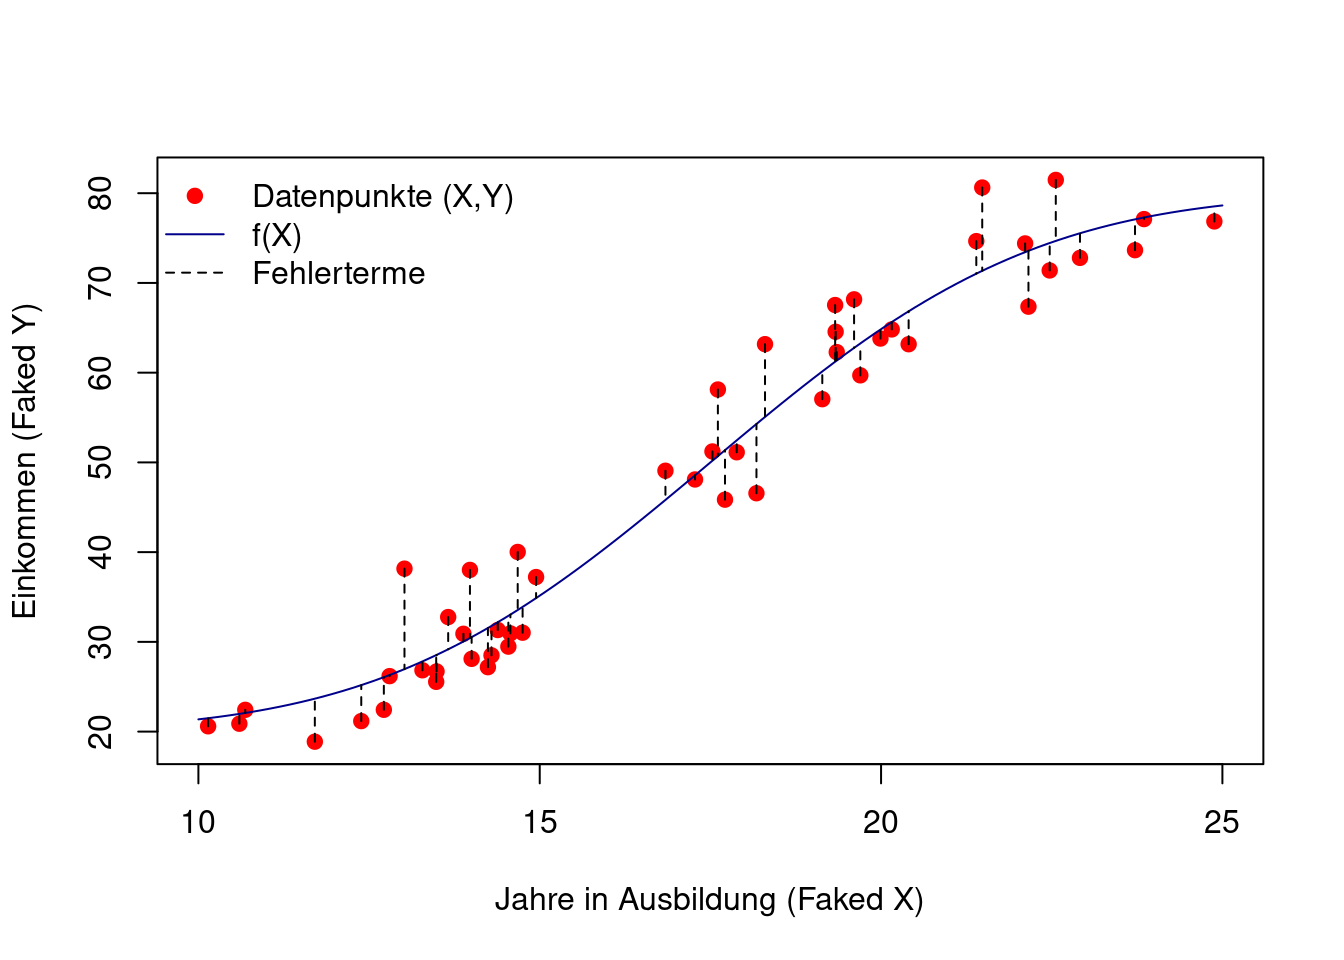
\includegraphics[width=0.9\linewidth]{Computational_Statistics_Script_files/figure-latex/fakedata-1} 

}

\caption{Simulierte (künstlich erzeugte) Daten zur Veranschaulichung einer allgemeinen, univariaten Regressionsbeziehung.}\label{fig:fakedata}
\end{figure}

Abbildung \ref{fig:plot3d} zeigt ein simuliertes Beispiel einer allgemeinen, bivariaten Regressionsbeziehung
\[
Y=f(X)+\varepsilon\quad\text{mit}\quad X=(X_1,X_2).
\]\\

\begin{figure}[h]

{\centering 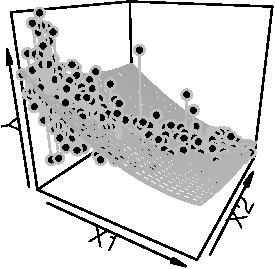
\includegraphics[width=5\linewidth,height=5\textheight]{Computational_Statistics_Script_files/figure-latex/plot3d-1} 

}

\caption{Veranschaulichung einer allgemeinen, bivariaten Regressionsbeziehung.}\label{fig:plot3d}
\end{figure}

\hypertarget{der-pruxe4diktionsfehler-zwischen-y-und-haty}{%
\subsection{\texorpdfstring{Der Prädiktionsfehler (zwischen \(Y\) und \(\hat{Y}\))}{Der Prädiktionsfehler (zwischen Y und \textbackslash hat\{Y\})}}\label{der-pruxe4diktionsfehler-zwischen-y-und-haty}}

In vielen Datenproblemen sind zwar die Prädiktorvariablen \(X\) bekannt (z.B. Gewicht, PS und Hubraum eines neuen Autos), aber die dazugehörige Zielvariable \(Y\) ist unbekannt. Da sich der Fehlerterm zu Null mittelt, lässt sich in solch einem Fall das unbekannte \(Y\) durch
\[
\hat{Y}=\hat{f}(X)
\]
vorhersagen, wobei

\begin{itemize}
\tightlist
\item
  \(\hat{f}\) für unsere Schätzung von \(f\) steht und
\item
  \(\hat{Y}\) die Vorhersage von \(Y\) für gegebene Prädiktorvariablen \(X\) ist.
\end{itemize}

Die Genauigkeit der Vorhersage von \(\hat{Y}\) für \(Y\) hängt von zwei verschiedenen Prädiktionsfehlergrößen ab:

\begin{itemize}
\tightlist
\item
  \textbf{Reduzierbarer Prädiktionsfehler} aufgrund des Schätzfehlers in \(\hat{f}\). Eine genauere Schätzung kann diesen Fehler reduzieren.
\item
  \textbf{Nicht reduzierbarer Prädiktionsfehler} aufgrund des Fehlerterms \(\varepsilon\). Das ist der Fehler, den wir selbst bei perfekter Schätzung von \(f\) nicht reduzieren können.
\end{itemize}

Der \textbf{nicht reduzierbare Fehler} \(\varepsilon\) enthält alle nicht messbaren und nicht gemessenen Variablen, die ebenfalls einen Einfluss auf \(Y\) haben. Und da wir diese Variablen nicht messen können, können wir sie auch nicht verwenden, um \(f\) zu schätzen.

Sei nun \(\hat{f}\) eine gegebene Schätzung von \(f\) und seien \(X\) gegeben Werte der Prädiktorvariablen welche die Vorhersage \(\hat{Y}=\hat{f}(X)\) ergeben. Nehmen wir nun für einen Moment an, dass \(\hat{f}\) und \(X\) gegeben und fest (also nicht zufällig) sind, dann
\begin{align*}
E\left[(Y-\hat{Y})^2\right]
&=E\Big[(\overbrace{f(X)+\varepsilon}^{=Y} - \overbrace{\hat{f}(X)}^{=\hat{Y}})^2\Big]\\
&=E\left[\left((f(X)-\hat{f}(X)\right)^2+2\left((f(X)-\hat{f}(X)\right)\varepsilon+\varepsilon^2\right]\\
&=\underbrace{\left((f(X)-\hat{f}(X)\right)^2}_{\text{reduzierbar}}+\underbrace{\operatorname{Var}(\varepsilon)}_{\text{nicht reduzierbar}}
\end{align*}
Der mittlere quadratische Prädiktionsfehler \(E\left[(Y-\hat{Y})^2\right]\) lässt sich also in eine reduzierbare und eine nicht reduzierbare Fehlerkomponente zerlegen.

\hypertarget{das-multivariate-lineare-regressionsmodell}{%
\section{Das multivariate lineare Regressionsmodell}\label{das-multivariate-lineare-regressionsmodell}}

Um die allgemeine Regressionsfunktion \(f(X)=E(Y|X)\) mit Hilfe der Daten zu schätzen (lernen), gibt es sehr viele verschiedenen Möglichkeiten. Eine der erfolgreichsten und am häufigsten verwendete Möglichkeit ist das \textbf{multivariaten linear Regressionsmodell}. Dieses Modell ist die \textbf{strukturelle Modellannahme}, dass sich die unbekannte Regressionsfunktion \(f\) als lineare Funktion (linear in den Modellparametern \(\beta_0, \beta_1, \dots, \beta_p\)) schreiben lässt:
\[
f(X)=\beta_0+\beta_1X_1+\dots+\beta_pX_p.
\]

Unter dieser Modellannahme wird das allgemeine Regressionsmodell \(Y=f(X)+\varepsilon\) zum multivariaten (multiplen) linearen Regressionsmodell
\begin{align*}
Y=\beta_0+\beta_1X_1+\dots+\beta_pX_p+\varepsilon.
\end{align*}
Zusammen mit der Annahme, dass \(\varepsilon\) unabhängig von \(X\) ist, und dass \(E(\varepsilon)=0\), können wir mit dieser Modellannahme den unbekannten bedingten Mittelwert \(E(Y|X)=f(X)\) vereinfacht schreiben als
\begin{align*}
E(Y|X)=\beta_0+\beta_1X_1+\dots+\beta_pX_p.
\end{align*}

Vorteile des \textbf{multivariaten linearen Regressionsmodells:}

\begin{itemize}
\tightlist
\item
  Anstatt eine gänzlich unbekannte Funktion \(f\) schätzen (lernen) zu müssen, muss man lediglich die unbekannten Parameterwerte \(\beta_0, \beta_1, \dots, \beta_p\) schätzen.
\item
  Die Modellstruktur ist \textbf{keine Black Box}, sondern gibt Aufschluss über die \textbf{assoziativen Zusammenhänge} zwischen den Prädiktorvariablen und der Zielvariablen.
\item
  Die lineare Modellstruktur ist \textbf{extrem flexibel}, da Transformationen der Prädiktorvariablen grundsätzlich erlaubt sind.
\end{itemize}

\begin{quote}
Gerade die große Flexibilität linearer Modelle werden wir nutzten müssen, um die \textbf{nicht linearen Zusammenhänge} zwischen den Prädiktorvariablen und der Zielvariablen in unserem Benzinverbrauchsbeispiel berücksichtigen zu können (siehe Abbildung \ref{fig:pairsplot}).
\end{quote}

\hypertarget{schuxe4tzung}{%
\subsection{Schätzung}\label{schuxe4tzung}}

Wir wollen nun diejenige Funktion
\[
\hat{f}(X)=\hat{\beta}_0 + \hat{\beta}_1 X_1 + \dots + \hat{\beta}_p X_p
\]
finden, sodass \(Y\approx \hat{f}(X)\) für alle Datenpunkte \((Y,X)\).

Zur Berechnung von \(\hat{f}\) können wir die \textbf{beobachteten Daten} als \textbf{Trainingsdaten} verwenden:
\[
\left\{(x_1,y_1),(x_2,y_2),\dots,(x_n,y_n)\right\}\quad\text{wobei}\quad x_i=(x_{i1},x_{i2},\dots,x_{ip})^T.
\]
Im Folgenden werden wir oft die Notation
\[x_{ij},\quad i=1,\dots,n,\quad j=1,\dots,p\]
verwenden, um die \(j\)te Prädiktorvariable der \(i\)ten Beobachtung zu bezeichnen. Der Laufindex \(j=1,\dots,p\) repräsentiert die einzelnen Prädiktorvariablen (z.B. Verbrauch, Gewicht, Pferdestärken, und Hubraum im \texttt{Auto\_df} Datensatz) und der Laufindex \(i=1,\dots,n\) repräsentiert die einzelnen Beobachtungen (z.B. gespeichert als Zeilen im \texttt{Auto\_df} Datensatz).

\begin{quote}
\textbf{Idee:} Die Trainingsdaten \(\left\{(x_1,y_1),(x_2,y_2),\dots,(x_n,y_n)\right\}\) enthalten Information zum unbekannten Regressionsmodell \(f\), da (so die Grundidee) die Daten von eben diesem Modell erzeugt wurden. Ziel ist also die unbekannte Regressionsfunktion \(f\) mit Hilfe der Trainingsdaten zu schätzen (erlernen).
\end{quote}

Für jede mögliche Schätzung \(\hat{f}\) von \(f\) können wir die beobachteten Werte der Zielvariablen \(y_i\) mit den vorhergesagten Werten
\[
\hat{y}_i=\hat{f}(x_i)=\hat{\beta}_0 + \hat{\beta}_1 x_{i1} +  \hat{\beta}_2 x_{i2} + \dots + \hat{\beta}_p x_{ip}
\]
vergleichen, indem wir die \textbf{Residuen}
\[
e_i = y_i-\hat{y}_i\quad i=1,\dots,n
\]
betrachten.

Die gängigste Methode zur Schätzung der unbekannten Modellparameter \(\beta_0,\beta_1,\dots,\beta_p\) ist die \textbf{Methode der kleinsten Quadrate}. Wir definieren die \textbf{Residuenquadratsumme} RSS (Residual Sum of Squares) als:
\[
\operatorname{RSS}=e_1^2+e_2^2+\dots +e_n^2
\]
oder äquivalent als
\[
\operatorname{RSS}=
(y_1-\hat{\beta}_0 + \hat{\beta}_1 x_{11} +  \dots + \hat{\beta}_p x_{1p})^2 + 
\dots +
(y_n-\hat{\beta}_0 + \hat{\beta}_1 x_{n1} +  \dots + \hat{\beta}_p x_{np})^2
\]
Die Methode der kleinsten Quadrate bestimmt die Parameterschätzungen \(\hat{\beta}=(\hat{\beta}_0,\hat{\beta}_1,\dots,\hat{\beta}_p)^T\) durch \textbf{Minimierung der Residuenquadratsumme RSS}. Nach ein paar Rechnungen kann man zeigen, dass\\
\begin{align*}
\left(
  \begin{matrix}
  \hat{\beta}_0\\
  \hat{\beta}_1\\
  \vdots\\
  \hat{\beta}_p
  \end{matrix}
\right)=
\left(
  \left(\begin{matrix}
  1&x_{11}&\dots & x_{1p}\\
  \vdots&&\ddots & \vdots\\
  1&x_{n1}&\dots & x_{np}\\
  \end{matrix}\right)^T
  \left(\begin{matrix}
  1&x_{11}&\dots & x_{1p}\\
  \vdots&&\ddots & \vdots\\
  1&x_{n1}&\dots & x_{np}\\
  \end{matrix}\right)
\right)^{-1}
\left(\begin{matrix}
  1&x_{11}&\dots & x_{1p}\\
  \vdots&&\ddots & \vdots\\
  1&x_{n1}&\dots & x_{np}\\
  \end{matrix}\right)^T
\left(
  \begin{matrix}
  Y_1\\
  \vdots\\
  Y_n
  \end{matrix}
\right)
\end{align*}

\hypertarget{polynomregression}{%
\subsection{Polynomregression}\label{polynomregression}}

Die \textbf{Polynomregression} ist eine Möglichkeit, die nicht linearen Beziehungen zwischen der Zielvariablen und den Prädiktorvariablen in unserem Benzinverbrauchsproblem (siehe Abbildung \ref{fig:pairsplot}) berücksichtigen zu können. So kann, zum Beispiel, der nicht lineare Zusammenhang zwischen \texttt{Verbrauch} und Leistung \texttt{PS} sehr flexibel als Polynomfunktion modelliert werden:
\[
\texttt{Verbrauch}=\beta_0 + \beta_1 \texttt{Ps} + \beta_2 \texttt{PS}^2 + \dots + \beta_p \texttt{PS}^p
\]
Je höher der Grad \(p\) des Polynoms, desto flexibler ist ein Polynomregressionsmodell und ermöglicht so auch die Modellierung nicht linearen Zusammenhänge. Das Polynomregressionsmodell ist jedoch für alle Polynomgrade \(p\) ein \textbf{(multivariates) lineares Regressionsmodell}, denn es ist linear bezüglich der Modellparameter \(\beta_0, \beta_1, \dots, \beta_p\).

\begin{Shaded}
\begin{Highlighting}[]
\DocumentationTok{\#\# Polynom Regressionen}
\NormalTok{polreg\_1 }\OtherTok{\textless{}{-}} \FunctionTok{lm}\NormalTok{(Verbrauch }\SpecialCharTok{\textasciitilde{}} \FunctionTok{poly}\NormalTok{(PS, }\AttributeTok{degree =} \DecValTok{1}\NormalTok{, }\AttributeTok{raw=}\ConstantTok{TRUE}\NormalTok{), }\AttributeTok{data =}\NormalTok{ Auto\_df)}
\NormalTok{polreg\_2 }\OtherTok{\textless{}{-}} \FunctionTok{lm}\NormalTok{(Verbrauch }\SpecialCharTok{\textasciitilde{}} \FunctionTok{poly}\NormalTok{(PS, }\AttributeTok{degree =} \DecValTok{2}\NormalTok{, }\AttributeTok{raw=}\ConstantTok{TRUE}\NormalTok{), }\AttributeTok{data =}\NormalTok{ Auto\_df)}
\NormalTok{polreg\_5 }\OtherTok{\textless{}{-}} \FunctionTok{lm}\NormalTok{(Verbrauch }\SpecialCharTok{\textasciitilde{}} \FunctionTok{poly}\NormalTok{(PS, }\AttributeTok{degree =} \DecValTok{5}\NormalTok{, }\AttributeTok{raw=}\ConstantTok{TRUE}\NormalTok{), }\AttributeTok{data =}\NormalTok{ Auto\_df)}
\DocumentationTok{\#\# Data{-}Frame zum Abspeichern der Prädiktionen}
\NormalTok{plot\_df       }\OtherTok{\textless{}{-}} \FunctionTok{tibble}\NormalTok{(}\StringTok{"PS"} \OtherTok{=} \FunctionTok{seq}\NormalTok{(}\DecValTok{45}\NormalTok{, }\DecValTok{250}\NormalTok{, }\AttributeTok{len=}\DecValTok{50}\NormalTok{))}
\DocumentationTok{\#\# Abspeichern der Prädiktionen}
\NormalTok{plot\_df}\SpecialCharTok{$}\NormalTok{fit\_1 }\OtherTok{\textless{}{-}} \FunctionTok{predict}\NormalTok{(polreg\_1, }\AttributeTok{newdata =}\NormalTok{ plot\_df)}
\NormalTok{plot\_df}\SpecialCharTok{$}\NormalTok{fit\_2 }\OtherTok{\textless{}{-}} \FunctionTok{predict}\NormalTok{(polreg\_2, }\AttributeTok{newdata =}\NormalTok{ plot\_df)}
\NormalTok{plot\_df}\SpecialCharTok{$}\NormalTok{fit\_5 }\OtherTok{\textless{}{-}} \FunctionTok{predict}\NormalTok{(polreg\_5, }\AttributeTok{newdata =}\NormalTok{ plot\_df)}
\DocumentationTok{\#\# Ploten}
\FunctionTok{plot}\NormalTok{(Verbrauch }\SpecialCharTok{\textasciitilde{}}\NormalTok{ PS, }\AttributeTok{data =}\NormalTok{ Auto\_df, }\AttributeTok{ylim=}\FunctionTok{c}\NormalTok{(}\DecValTok{2}\NormalTok{,}\DecValTok{20}\NormalTok{),}
     \AttributeTok{xlab=}\StringTok{"Leistung (PS)"}\NormalTok{, }\AttributeTok{pch=}\DecValTok{21}\NormalTok{, }\AttributeTok{col=}\StringTok{"gray"}\NormalTok{, }\AttributeTok{bg=}\StringTok{"gray"}\NormalTok{, }\AttributeTok{cex=}\FloatTok{1.5}\NormalTok{)}
\FunctionTok{with}\NormalTok{(plot\_df, }\FunctionTok{lines}\NormalTok{(}\AttributeTok{x =}\NormalTok{ PS, }\AttributeTok{y =}\NormalTok{ fit\_1, }\AttributeTok{lwd=}\DecValTok{2}\NormalTok{, }\AttributeTok{col=}\StringTok{"orange"}\NormalTok{))}
\FunctionTok{with}\NormalTok{(plot\_df, }\FunctionTok{lines}\NormalTok{(}\AttributeTok{x =}\NormalTok{ PS, }\AttributeTok{y =}\NormalTok{ fit\_2, }\AttributeTok{lwd=}\DecValTok{2}\NormalTok{, }\AttributeTok{col=}\StringTok{"blue"}\NormalTok{))}
\FunctionTok{with}\NormalTok{(plot\_df, }\FunctionTok{lines}\NormalTok{(}\AttributeTok{x =}\NormalTok{ PS, }\AttributeTok{y =}\NormalTok{ fit\_5, }\AttributeTok{lwd=}\DecValTok{2}\NormalTok{, }\AttributeTok{col=}\StringTok{"darkgreen"}\NormalTok{))}
\FunctionTok{legend}\NormalTok{(}\StringTok{"topright"}\NormalTok{, }\AttributeTok{lty=}\FunctionTok{c}\NormalTok{(}\ConstantTok{NA}\NormalTok{,}\DecValTok{1}\NormalTok{,}\DecValTok{1}\NormalTok{,}\DecValTok{1}\NormalTok{), }\AttributeTok{pch=}\FunctionTok{c}\NormalTok{(}\DecValTok{21}\NormalTok{,}\ConstantTok{NA}\NormalTok{,}\ConstantTok{NA}\NormalTok{,}\ConstantTok{NA}\NormalTok{), }
       \AttributeTok{col=}\FunctionTok{c}\NormalTok{(}\StringTok{"gray"}\NormalTok{,}\StringTok{"orange"}\NormalTok{,}\StringTok{"blue"}\NormalTok{,}\StringTok{"darkgreen"}\NormalTok{), }\AttributeTok{pt.bg=}\StringTok{"gray"}\NormalTok{, }\AttributeTok{pt.cex=}\FloatTok{1.5}\NormalTok{,}
       \AttributeTok{legend=}\FunctionTok{c}\NormalTok{(}\StringTok{"Datenpunkte"}\NormalTok{, }\StringTok{"Grad 1"}\NormalTok{, }\StringTok{"Grad 2"}\NormalTok{, }\StringTok{"Grad 5"}\NormalTok{), }\AttributeTok{bty=}\StringTok{"n"}\NormalTok{)}
\end{Highlighting}
\end{Shaded}

\begin{figure}[h]

{\centering 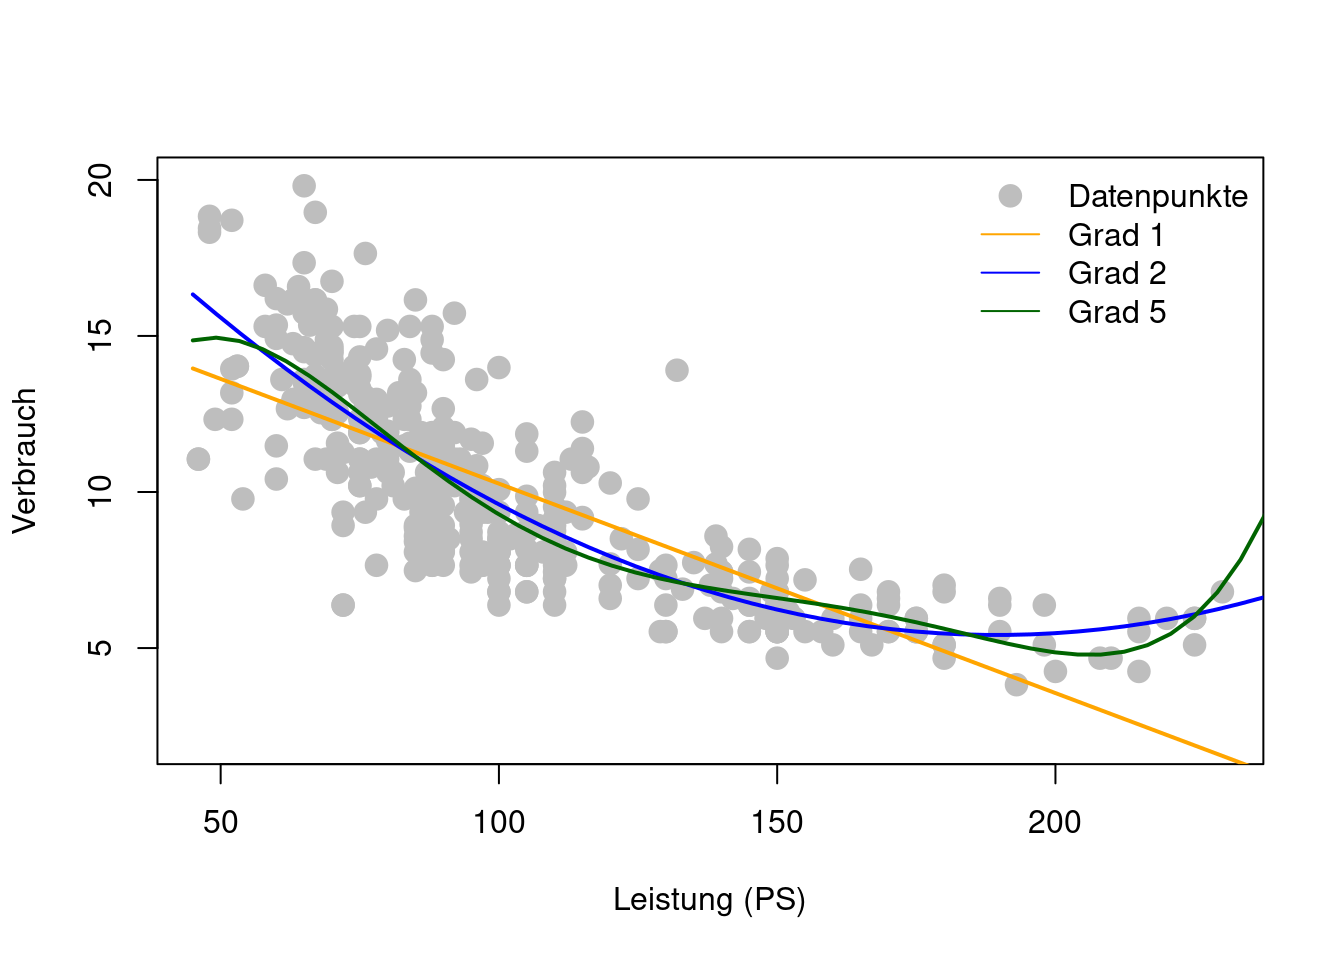
\includegraphics[width=1\linewidth,height=1\textheight]{Computational_Statistics_Script_files/figure-latex/polynom-1} 

}

\caption{Polynom Regression bei verschiedenen Polynomgraden $p$.}\label{fig:polynom}
\end{figure}

\hypertarget{uxfcberanpassung}{%
\subsubsection*{Überanpassung}\label{uxfcberanpassung}}
\addcontentsline{toc}{subsubsection}{Überanpassung}

Zusätzlich zur Wahl der Modellparameter \(\hat{\beta}_0, \hat{\beta}_1, \dots, \hat{\beta}_p\) besteht hier nun das Problem
der Wahl des Grades \(p\) des Polynoms als weiteren Modellparameter
\[
y_i=\hat{\beta}_0 + \hat{\beta}_1 x_{i1} + \hat{\beta}_2 x_{i2}^2 + \dots + \hat{\beta}_p x_{ip}^p + e_i
\]
Wenn man jedoch versucht, alle Modellparameter (also \(\hat{\beta}_0, \hat{\beta}_1, \dots, \hat{\beta}_p\) \textbf{und} \(p\)) durch Minimieren der Trainingsdaten-RSS
\[
\operatorname{RSS}\equiv\operatorname{RSS}(\hat{\beta}_0, \hat{\beta}_1, \dots, \hat{\beta}_p,p)=e_1^2 + e_2^2 + \dots + e_n^2
\]
zu schätzen, so ergibt sich ein Problem das als \textbf{Überanpassung} (\textbf{Overfitting}) bekannt ist (siehe Abbildung \ref{fig:RSSPoly2}). Das Polynomregressionsmodell ist so flexibel, dass es den einzelnen Trainingsdaten \((x_i,y_i)\) folgen kann. Eine Überangepassung an die Trainingsdaten führt jedoch notwendigerweise zu einer Verschlechterung der Vorhersagegüte bezüglich \emph{neuer} Daten.

\begin{figure}[h]

{\centering 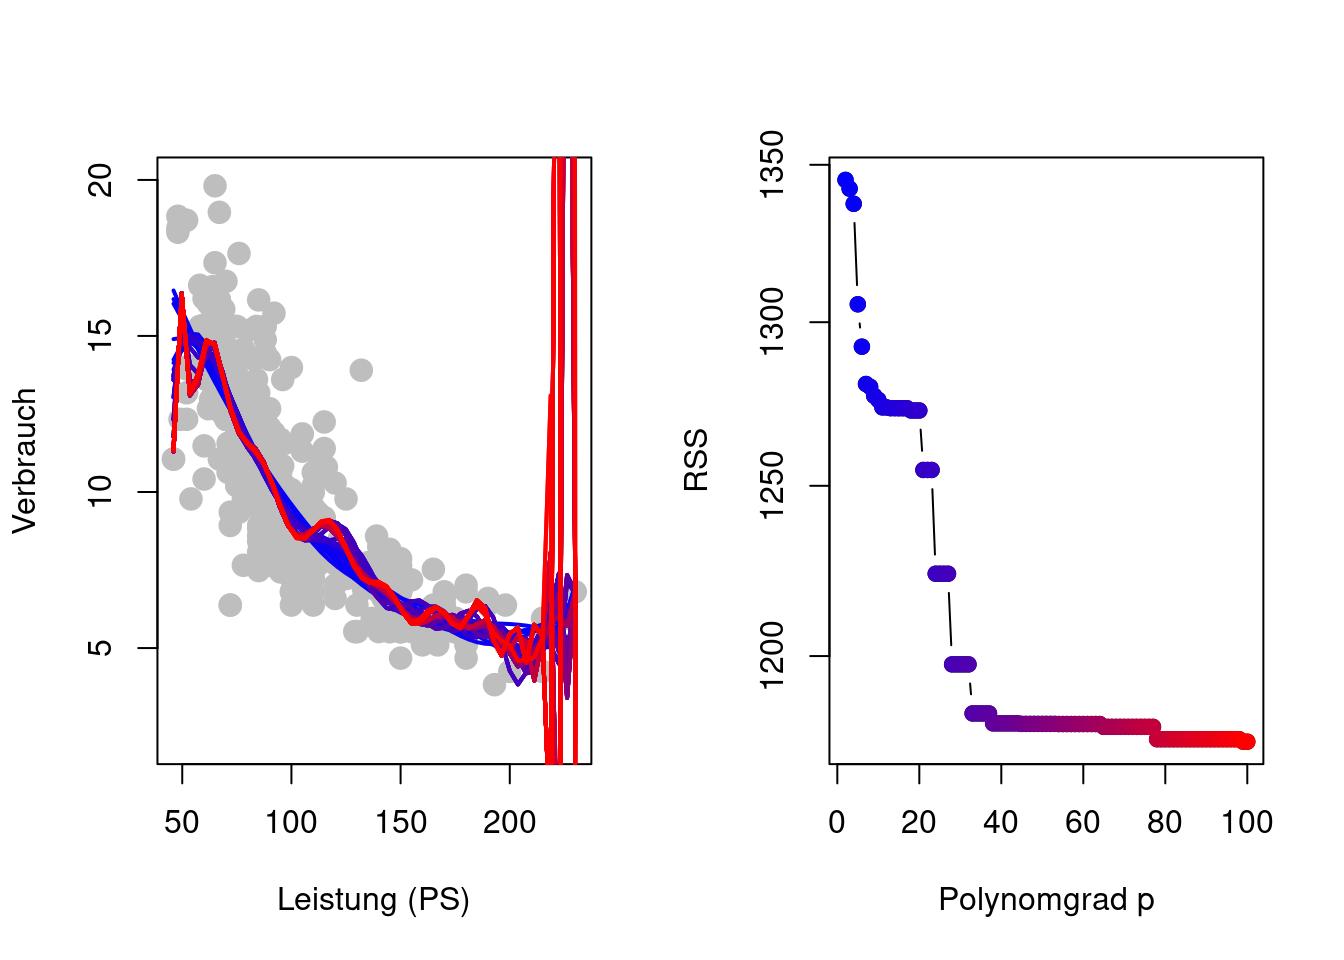
\includegraphics[width=0.9\linewidth]{Computational_Statistics_Script_files/figure-latex/RSSPoly2-1} 

}

\caption{Polynom Regression und die Wahl des Polynomgrades $p$ durch Minimierung der Trainingsdaten-RSS. (Eine schlechte Idee).}\label{fig:RSSPoly2}
\end{figure}

\hypertarget{modellauswahl}{%
\section{Modellauswahl}\label{modellauswahl}}

\hypertarget{maschinelles-lernen-versus-strukturelle-modelle}{%
\subsubsection*{Maschinelles Lernen versus Strukturelle Modelle}\label{maschinelles-lernen-versus-strukturelle-modelle}}
\addcontentsline{toc}{subsubsection}{Maschinelles Lernen versus Strukturelle Modelle}

Das oben veranschaulichte Problem der Überanpassung (Overfitting) ist eng damit verbunden, dass wir hier ein sehr flexibles Regressionsmodell (Polynomregression) betrachten. Viele der möglichen Polynomfunktionen sind unsinnig, da sie nicht die strukturellen Einschränkungen des betrachteten Datenproblems berücksichtigen. Falls ein gesichertes Wissen zu den zugrundeliegenden, strukturellen Zusammenhängen zwischen der Zielvariable \(Y\) und den Prädiktorvariablen \(X\) existiert, sollte man diese strukturellen Zusammenhängen auch im statistischen Modell berücksichtigen. (Immer mit den Expert*Innen des Faches sprechen!) Im besten Falle gibt es ein \textbf{strukturelles Modell} zu den systematischen Zusammenhängen \(f\) zwischen \(Y\) und \(X\), welches genügend Einschränkungen bietet, sodass alle unsinnigen Modellierungen vermieden werden können. In solchen Idealfällen führt die Minimierung der Trainingsdaten-RSS zu keinem Problem der Überanpassung.

Falls jedoch kein (vertrauenswürdiges) strukturelles Modell vorliegt, ist die Verwendung von sehr flexiblen Regressionsmodellen wie der Polynomregression eine grundsätzlich sehr gute Idee, da wir so, ohne große Einschränkungen, nach den unbekannten richtigen Zusammenhängen \(f\) suchen können. Dies ist der Ansatz des \textbf{maschinellen Lernens} und die \textbf{Polynomregression mit unbekanntem Polynomgrad \(p\)} ist lediglich eine von sehr vielen Methoden, welche im Kontext des maschinellen Lernens verwendet werden.

\begin{quote}
\textbf{Fazit:} Methoden des \textbf{maschinellen Lernens} sind typischerweise sehr flexibel und bauen nicht auf strukturellen Modellen auf. Daher benötigen diese Methoden spezielle Verfahren der \textbf{Modellauswahl}, um eine Überanpassung an die Trainingsdaten zu vermeiden. Richtig angewandt, können Methoden des maschinellen Lernens unbekannte Zusammenhänge richtig erkennen.
\end{quote}

\hypertarget{die-validierungsdaten-methode}{%
\subsection{Die Validierungsdaten-Methode}\label{die-validierungsdaten-methode}}

Da die Minimierung der Trainingsdaten-RSS schnell zu einem Problem der Überanpassung führt, benötigen wir eine alternative Methode, um die Güte des geschätzten Modells zu prüfen. Die einfachste Idee ist dabei die beobachteten Daten in einen Satz von Trainingsdaten
\[
\text{Trainingsdaten}=\left\{(x_{1}^{Train},y_{1}^{Train}), (x_{2}^{Train},y_{2}^{Train}),\dots,(x_{n_{Train}}^{Train},y_{n_{Train}}^{Train})\right\}
\]
und einen \textbf{separaten} (disjunkten) Satz von Validierungsdaten
\[
\text{Validierungsdaten}=\left\{(x_{1}^{Valid},y_{1}^{Valid}), (x_{2}^{Valid},y_{2}^{Valid}),\dots,(x_{n_{Valid}}^{Valid},y_{n_{Valid}}^{Valid})\right\}
\]
zu teilen mit

\begin{itemize}
\tightlist
\item
  \(n=n_{Train} + n_{Valid}\)
\item
  \(\text{Trainingsdaten}\cap \text{Validierungsdaten} = \emptyset\)
\end{itemize}

Folgender Code-Schnipsel ermöglicht solch eine (zufällige) Aufteilung der Daten in Trainings- und Validierungsdaten:

\begin{Shaded}
\begin{Highlighting}[]
\NormalTok{n        }\OtherTok{\textless{}{-}} \FunctionTok{nrow}\NormalTok{(Auto\_df) }\CommentTok{\# Stichprobenumfang}
\NormalTok{n\_Train  }\OtherTok{\textless{}{-}} \DecValTok{200}           \CommentTok{\# Stichprobenumfang der Trainingsdaten}
\NormalTok{n\_Valid  }\OtherTok{\textless{}{-}}\NormalTok{ n }\SpecialCharTok{{-}}\NormalTok{ n\_Train   }\CommentTok{\# Stichprobenumfang der Validierungsdaten}

\DocumentationTok{\#\# Index{-}Mengen zur Auswahl der }
\DocumentationTok{\#\# Trainings{-} und Validierungsdaten}
\NormalTok{I\_Train  }\OtherTok{\textless{}{-}} \FunctionTok{sample}\NormalTok{(}\AttributeTok{x =} \DecValTok{1}\SpecialCharTok{:}\NormalTok{n, }\AttributeTok{size =}\NormalTok{ n\_Train, }\AttributeTok{replace =} \ConstantTok{FALSE}\NormalTok{)}
\NormalTok{I\_Valid  }\OtherTok{\textless{}{-}} \FunctionTok{c}\NormalTok{(}\DecValTok{1}\SpecialCharTok{:}\NormalTok{n)[}\SpecialCharTok{{-}}\NormalTok{I\_Train]}

\DocumentationTok{\#\# Trainingsdaten }
\NormalTok{Auto\_Train\_df }\OtherTok{\textless{}{-}}\NormalTok{ Auto\_df[I\_Train, ]}
\DocumentationTok{\#\# Validierungsdaten }
\NormalTok{Auto\_Valid\_df }\OtherTok{\textless{}{-}}\NormalTok{ Auto\_df[I\_Valid, ]}
\end{Highlighting}
\end{Shaded}

Obschon die Validierungsdaten-Methode auf alle Regressionsmodelle angewandt werden kann, veranschaulichen wir im Folgenden die Methode anhand der Polynomregression.

Die Aufteilung der Daten in Trainings- und Validierungsdaten ermöglicht uns nun ein zweistufiges Verfahren:

\textbf{Schritt 1:} Mit Hilfe der \textbf{Trainingsdaten} wird das Polynomregressionsmodell \textbf{geschätzt}:
\begin{align*}
y^{Train}_i
%&=\hat{f}^{Train}_p(x_i^{Train}) + e_i^{Train}\\
&=\hat{\beta}_0^{Train} + \hat{\beta}_1^{Train} x_{i}^{Train} + \hat{\beta}_2^{Train} (x_{i}^{Train})^2 + \dots + \hat{\beta}_p^{Train} (x_{i}^{Train})^p + e_i^{Train}
\end{align*}
Code-Schnipsel Beispiel:

\begin{Shaded}
\begin{Highlighting}[]
\NormalTok{Train\_polreg }\OtherTok{\textless{}{-}} \FunctionTok{lm}\NormalTok{(Verbrauch }\SpecialCharTok{\textasciitilde{}} \FunctionTok{poly}\NormalTok{(PS, }\AttributeTok{degree =}\NormalTok{ p, }\AttributeTok{raw=}\ConstantTok{TRUE}\NormalTok{), }\AttributeTok{data =}\NormalTok{ Auto\_Train\_df)}
\end{Highlighting}
\end{Shaded}

\textbf{Schritt 2:} Mit Hilfe der \textbf{Validierungsdaten} wird das geschätzte Polynomregressionsmodell \textbf{validiert}:
\begin{align*}
\hat{y}^{Valid}_i
%&=\hat{f}_p^{Train}(x_i^{Valid})+ e_i^{Valid}\\
&=\hat{\beta}_0 + \hat{\beta}_1^{Train} x_{i}^{Valid} + \hat{\beta}_2^{Train} (x_{i}^{Valid})^2 + \dots + \hat{\beta}_p^{Train} (x_{i}^{Valid})^p,
\end{align*}
indem man den \textbf{mittleren quadratischen Prädiktionsfehler} (Mean Squared Prediction Error \textbf{MSPE}) berechnet:
\begin{align*}
\text{MSPE}
&=\frac{1}{n_{Valid}}\text{RSS}_{Valid}\\
&=\frac{1}{n_{Valid}}\left((y_1^{Valid} - \hat{y}_1^{Valid})^2 +\dots + (y_{n_{Valid}}^{Valid} - \hat{y}_{n_{Valid}}^{Valid})^2\right)
\end{align*}
Code-Schnipsel Beispiel:

\begin{Shaded}
\begin{Highlighting}[]
\NormalTok{y\_fit\_Valid   }\OtherTok{\textless{}{-}} \FunctionTok{predict}\NormalTok{(Train\_polreg, }\AttributeTok{newdata =}\NormalTok{ Auto\_Valid\_df)}
\NormalTok{RSS\_Valid     }\OtherTok{\textless{}{-}} \FunctionTok{sum}\NormalTok{( (Auto\_Valid\_df}\SpecialCharTok{$}\NormalTok{Verbrauch }\SpecialCharTok{{-}}\NormalTok{ y\_fit\_Valid)}\SpecialCharTok{\^{}}\DecValTok{2}\NormalTok{ )}
\NormalTok{MSPE          }\OtherTok{\textless{}{-}}\NormalTok{ RSS\_Valid }\SpecialCharTok{/}\NormalTok{ n\_Valid}
\end{Highlighting}
\end{Shaded}

Man wiederholt obige Schritte für eine Auswahl von verschiedenen Polynomgraden \(p=1,2,\dots,p_{\max}\), z.B. \(p_{\max}=10\), und berechnet für jeden dieser Fälle den \(\operatorname{MSPE}\), also:
\[
\operatorname{MSPE}\equiv\operatorname{MSPE}(\hat{\beta}_0, \hat{\beta}_1, \dots, \hat{\beta}_p,p),\quad\text{für jedes}\quad p=1,2,\dots,p_{\max}
\]
Der \(\operatorname{MSPE}\) ist eine Schätzung des wahren, unbekannten mittleren quadratischen Prädiktionsfehlers \(E\left[(Y-\hat{Y})^2\right]\),\\
\[
\operatorname{MSPE}(\hat{\beta}_0, \hat{\beta}_1, \dots, \hat{\beta}_p,p)\approx E\left[(Y-\hat{Y})^2\right]. 
\]
Die Minimierung des \(\operatorname{MSPE}\) über verschiedene Werte des Polynomgrades \(p=1,2,\dots\) erlaubt es uns den \textbf{reduzierbaren Prädiktions-Fehler} der Polynomregression zu minimieren.

Folgender R-Code verbindet nun alle Schritte und berechnet den \(\operatorname{MSPE}\) für verschiedene Werte des Polynomgrades \(p\). Dasjenige Modell, welches den \(\operatorname{MSPE}\) minimiert, ist laut der Daten das beste Prädiktionsmodell.

\begin{Shaded}
\begin{Highlighting}[]
\FunctionTok{set.seed}\NormalTok{(}\DecValTok{31}\NormalTok{)}
\DocumentationTok{\#\#}
\NormalTok{n        }\OtherTok{\textless{}{-}} \FunctionTok{nrow}\NormalTok{(Auto\_df) }\CommentTok{\# Stichprobenumfang}
\NormalTok{n\_Train  }\OtherTok{\textless{}{-}} \DecValTok{200}           \CommentTok{\# Stichprobenumfang der Trainingsdaten}
\NormalTok{n\_Valid  }\OtherTok{\textless{}{-}}\NormalTok{n }\SpecialCharTok{{-}}\NormalTok{ n\_Train    }\CommentTok{\# Stichprobenumfang der Validierungsdaten}

\DocumentationTok{\#\# Index{-}Mengen zur Auswahl der }
\DocumentationTok{\#\# Trainings{-} und Validierungsdaten}
\NormalTok{I\_Train  }\OtherTok{\textless{}{-}} \FunctionTok{sample}\NormalTok{(}\AttributeTok{x =} \DecValTok{1}\SpecialCharTok{:}\NormalTok{n, }\AttributeTok{size =}\NormalTok{ n\_Train, }\AttributeTok{replace =} \ConstantTok{FALSE}\NormalTok{)}
\NormalTok{I\_Valid  }\OtherTok{\textless{}{-}} \FunctionTok{c}\NormalTok{(}\DecValTok{1}\SpecialCharTok{:}\NormalTok{n)[}\SpecialCharTok{{-}}\NormalTok{I\_Train]}

\DocumentationTok{\#\# Trainingsdaten }
\NormalTok{Auto\_Train\_df }\OtherTok{\textless{}{-}}\NormalTok{ Auto\_df[I\_Train, ]}
\DocumentationTok{\#\# Validierungsdaten }
\NormalTok{Auto\_Valid\_df }\OtherTok{\textless{}{-}}\NormalTok{ Auto\_df[I\_Valid, ]}

\NormalTok{p\_max         }\OtherTok{\textless{}{-}} \DecValTok{6}
\NormalTok{MSPE          }\OtherTok{\textless{}{-}} \FunctionTok{numeric}\NormalTok{(p\_max)}
\NormalTok{fit\_plot      }\OtherTok{\textless{}{-}} \FunctionTok{matrix}\NormalTok{(}\ConstantTok{NA}\NormalTok{, }\DecValTok{50}\NormalTok{, p\_max)}
\ControlFlowTok{for}\NormalTok{(p }\ControlFlowTok{in} \DecValTok{1}\SpecialCharTok{:}\NormalTok{p\_max)\{}
  \DocumentationTok{\#\# Schritt 1}
\NormalTok{  Train\_polreg }\OtherTok{\textless{}{-}} \FunctionTok{lm}\NormalTok{(Verbrauch }\SpecialCharTok{\textasciitilde{}} \FunctionTok{poly}\NormalTok{(PS, }\AttributeTok{degree =}\NormalTok{ p, }\AttributeTok{raw=}\ConstantTok{TRUE}\NormalTok{), }
                     \AttributeTok{data =}\NormalTok{ Auto\_Train\_df)}
  \DocumentationTok{\#\# Schritt 2}
\NormalTok{  y\_fit\_Valid   }\OtherTok{\textless{}{-}} \FunctionTok{predict}\NormalTok{(Train\_polreg, }\AttributeTok{newdata =}\NormalTok{ Auto\_Valid\_df)}
\NormalTok{  RSS\_Valid     }\OtherTok{\textless{}{-}} \FunctionTok{sum}\NormalTok{( (Auto\_Valid\_df}\SpecialCharTok{$}\NormalTok{Verbrauch }\SpecialCharTok{{-}}\NormalTok{ y\_fit\_Valid)}\SpecialCharTok{\^{}}\DecValTok{2}\NormalTok{ )}
\NormalTok{  MSPE[p]       }\OtherTok{\textless{}{-}}\NormalTok{ RSS\_Valid }\SpecialCharTok{/}\NormalTok{ n\_Valid}
  \DocumentationTok{\#\# Daten für\textquotesingle{}s plotten}
\NormalTok{  fit\_plot[,p] }\OtherTok{\textless{}{-}} \FunctionTok{predict}\NormalTok{(Train\_polreg, }\AttributeTok{newdata =}\NormalTok{ plot\_df)}
\NormalTok{\}}
\end{Highlighting}
\end{Shaded}

\begin{figure}[h]

{\centering 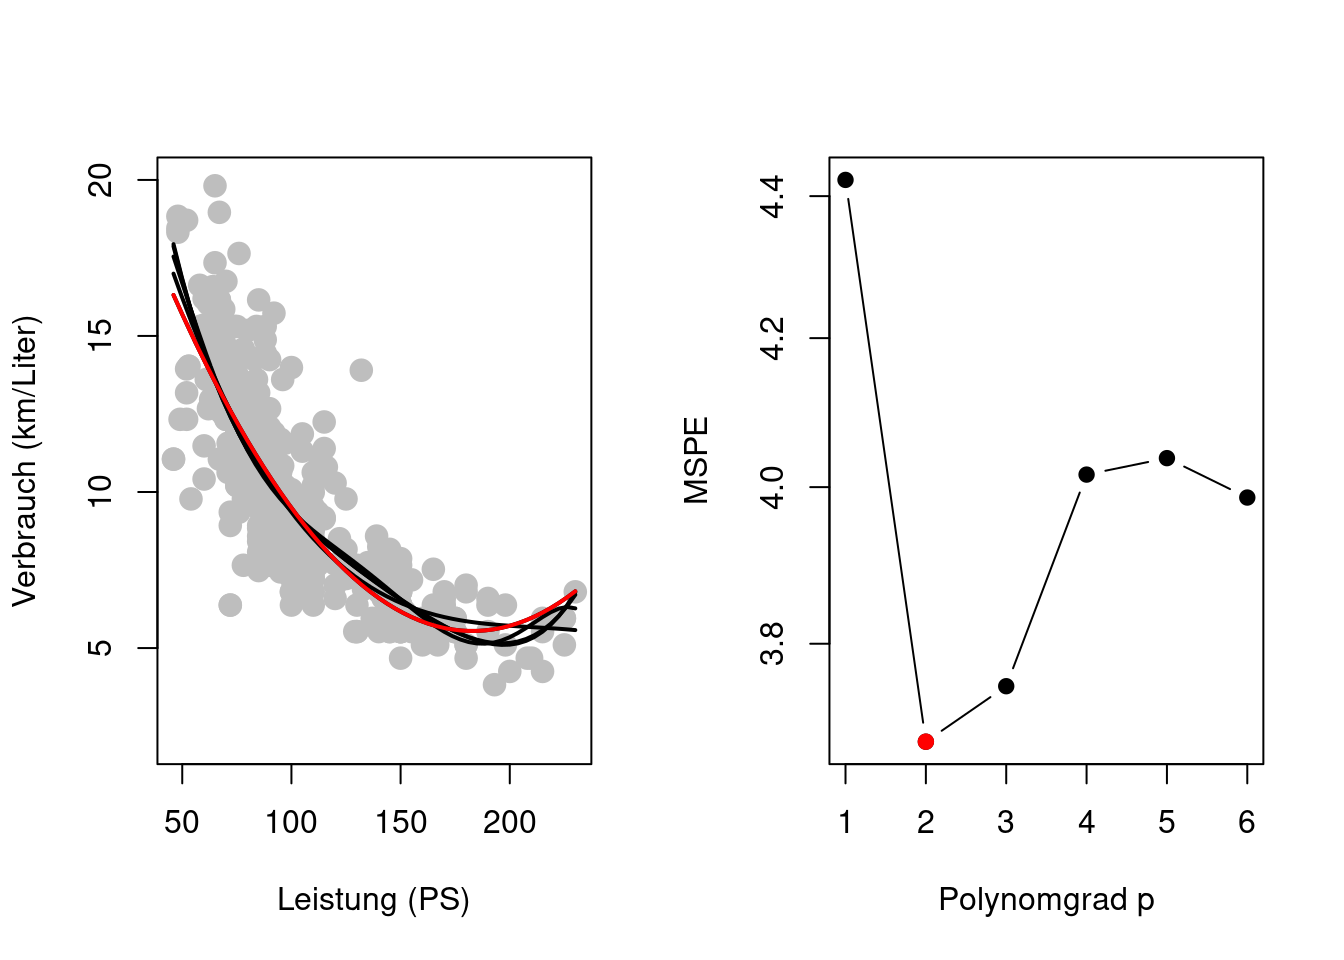
\includegraphics[width=0.9\linewidth]{Computational_Statistics_Script_files/figure-latex/RSSPoly3-1} 

}

\caption{Polynom Regression und die Wahl des Polynomgrades $p$ durch Minimierung des mittleren quadratischen Prädiktionsfehler MSPE.}\label{fig:RSSPoly3}
\end{figure}

\begin{quote}
\textbf{Achtung:} Auch eine Modellauswahl ist fehlerhaft und stellt lediglich eine Schätzung (mit Schätzfehlern) des besten Prädiktionsmodelles innerhalb der betrachteten Klasse von Prädiktionsmodellen (hier Polynomregressionen) dar.
\end{quote}

Abbildung \ref{fig:MSPE} zeigt jedoch ein Problem der Validierungsdaten-Methode. Die Trainingsdaten und die Validierungsdaten haben kleinere Stichprobenumfänge (\(n_{Train}<n\) und \(n_{Valid}<n\)) was zu einer \textbf{erhöhten Schätzgenauigkeit in der MSPE-Schätzung} führt.

\begin{figure}[h]

{\centering 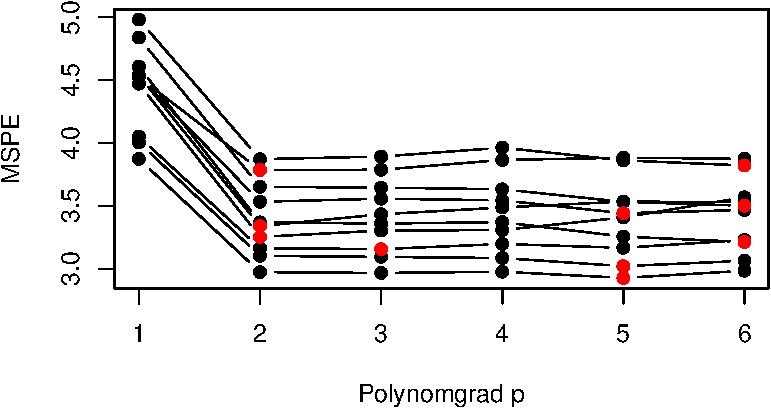
\includegraphics[width=0.9\linewidth]{Computational_Statistics_Script_files/figure-latex/MSPE-1} 

}

\caption{Zehn verschiedene MSPE-Berechnungen basierend auf zehn verschiedenen, zufälligen Aufteilungen der Daten in Trainings- und Validierungsdaten.}\label{fig:MSPE}
\end{figure}

\hypertarget{k-fache-kreuzvalidierung}{%
\subsection{k-Fache Kreuzvalidierung}\label{k-fache-kreuzvalidierung}}

Die \(k\)-fache (z.B. \(k=5\) oder \(k=10\)) Kreuzvalidierung ist eine Vorgehensweise zur Bewertung der Leistung einer Schätzprozedur (Algorithmus) im Kontext des maschinellen Lernens. Als Schätzprozedur verwenden wir wieder das Beispiel der Polynomregression mit unbekanntem Polynomgrad \(p\), welcher zusammen mit den Modellparametern \(\beta_0,\beta_1,\dots,\beta_p\) aus den Daten erlernt werden muss.

Die \(k\)-fache Kreuzvalidierung stellt eine Verbesserung der Validierungsdaten-Methode dar, da sie faktisch die Stichprobenumfänge in den Trainingsdaten und Validierungsdaten erhöht. Wie bei der Validierungsdaten-Methode wird der Datensatz in Trainings- und Validierungsdaten aufgeteilt -- jedoch \(k\)-fach. Abbildung \ref{fig:kfoldcv} zeigt ein Beispiel der Datenaufteilung bei der \(5\)-fachen Kreuzvalidierung.

Folgender Code-Schnipsel ermöglicht eine (zufällige) Aufteilung der Daten in \(k\) verschiedene Trainings- und Validierungsdaten:

\begin{Shaded}
\begin{Highlighting}[]
\NormalTok{n      }\OtherTok{\textless{}{-}} \FunctionTok{nrow}\NormalTok{(Auto\_df) }\CommentTok{\# Stichprobenumfang}
\NormalTok{k      }\OtherTok{\textless{}{-}} \DecValTok{5}             \CommentTok{\# 5{-}fache Kreuzvalidierung}

\DocumentationTok{\#\# Index zur Auswahl k verschiedener  }
\DocumentationTok{\#\# Trainings{-} und Validierungsdaten:}
\NormalTok{folds  }\OtherTok{\textless{}{-}} \FunctionTok{sample}\NormalTok{(}\AttributeTok{x =} \DecValTok{1}\SpecialCharTok{:}\NormalTok{k, }\AttributeTok{size =}\NormalTok{ n, }\AttributeTok{replace=}\ConstantTok{TRUE}\NormalTok{)}

\DocumentationTok{\#\# Trainingsdaten im j{-}ten (j=1,2,...,k) Durchgang}
\NormalTok{Auto\_df[folds }\SpecialCharTok{!=}\NormalTok{ j,]}
\DocumentationTok{\#\# Validierungsdaten im j{-}ten (j=1,2,...,k) Durchgang}
\NormalTok{Auto\_df[folds }\SpecialCharTok{==}\NormalTok{ j,]}
\end{Highlighting}
\end{Shaded}

Für jede der \(k\) Datenaufteilungen wird der \(\operatorname{MSPE}\) berechnet. Der Mittelwert dieser MSPE-Werte wird häufig als \(\operatorname{CV}_{(k)}\) Wert (crossvalidation score) bezeichnet
\[
\operatorname{CV}_{(k)}=\frac{1}{k}\sum_{j=1}^k\operatorname{MSPE}_j
\]

Der \(\operatorname{CV}_{(k)}\)-Wert stellt eine im Vergleich zur Validierungsdaten-Methode verbesserte Schätzung des unbekannten mittleren quadratischen Pädiktionsfehlers \(\operatorname{CV}_{(k)}\approx E[(Y-\hat{Y})^2]\) dar. Die Modellauswahl folgt also auch hier mittels Minimierung des \(\operatorname{CV}_{(k)}\)-Wertes über die verschiedene Werte des Polynomgrades \(p=1,2,\dots\).

\begin{quote}
\textbf{Wahl von \(k\):} In der Praxis haben sich die Werte \(k=5\) und \(k=10\) etabliert, da diese Größenordnunen einen guten Kompromiss zwischen der Varianz und der Verzerrung des Schätzers \(\operatorname{CV}_{(k)}\) für \(E[(Y-\hat{Y})^2]\) darstellen.
\end{quote}

\hypertarget{anwendung-vorhersage-des-benzinverbrauchs}{%
\section{Anwendung: Vorhersage des Benzinverbrauchs}\label{anwendung-vorhersage-des-benzinverbrauchs}}

Nun haben wir das Werkzeug, um die nicht linearen Zusammenhänge zwischen der \textbf{Zielvariable} \(Y=\)\texttt{Verbrauch} und den \textbf{Prädiktorvariablen} \(G=\)\texttt{Gewicht}, \(P=\)\texttt{PS} und \(H=\)\texttt{Hubraum} im Datensatz \texttt{Auto\_df} zu berücksichtigen (siehe Abbildung \ref{fig:pairsplot}) und allein mit Hilfe der Daten zu erlernen. Wir folgen hier der Herangehensweise des \textbf{maschinellen Lernens} und lassen die \textbf{Daten für sich selbst sprechen}.

Da Abbildung \ref{fig:pairsplot} sehr ähnliche Zusammenhänge zwischen der Zielvariable \(Y=\)\texttt{Verbrauch} und den Prädiktorvariablen \(G=\)\texttt{Gewicht}, \(P=\)\texttt{PS} und \(H=\)\texttt{Hubraum} vermuten lässt, betrachten wir zunächst ein vereinfachtest Polynomregressionsmodell, bei dem für alle Prädiktorvariablen der gleiche Polynomgrad \(p\) verwendet wird.\\
\begin{align*}
Y_i = \beta_0 + \notag
& \beta^G_{1} G_i + \beta^G_{2} G_i^2 + \dots + \beta^G_{p} G_i^p + \\
& \beta^P_{1} P_i + \beta^P_{2} P_i^2 + \dots + \beta^P_{p} P_i^p +  \\
& \beta^H_{1} H_i + \beta^H_{2} H_i^2 + \dots + \beta^H_{p} H_i^p +  \varepsilon_i 
\end{align*}

Folgender R-Code (Algorithmus) erlernt aus den Daten, mit Hilfe der \(5\)-fachen Kreuzvalidierung \(\operatorname{CV}_{(5)}\approx E[(Y-\hat{Y})^2]\), den optimalen Polynomgrad \(p\).

\begin{Shaded}
\begin{Highlighting}[]
\FunctionTok{set.seed}\NormalTok{(}\DecValTok{8}\NormalTok{)             }\CommentTok{\# Seed für den Zufallsgenerator}

\NormalTok{n      }\OtherTok{\textless{}{-}} \FunctionTok{nrow}\NormalTok{(Auto\_df) }\CommentTok{\# Stichprobenumfang}
\NormalTok{k      }\OtherTok{\textless{}{-}} \DecValTok{5}             \CommentTok{\# 5{-}fache Kreuzvalidierung}
\NormalTok{p\_max  }\OtherTok{\textless{}{-}} \DecValTok{5}             \CommentTok{\# Maximaler Polynomgrad}

\NormalTok{folds     }\OtherTok{\textless{}{-}} \FunctionTok{sample}\NormalTok{(}\AttributeTok{x =} \DecValTok{1}\SpecialCharTok{:}\NormalTok{k, }\AttributeTok{size =}\NormalTok{ n, }\AttributeTok{replace=}\ConstantTok{TRUE}\NormalTok{)}

\DocumentationTok{\#\# Container für die MSPE{-}Werte }
\DocumentationTok{\#\# für alle j=1,...,k Kreuzvalidierungen und }
\DocumentationTok{\#\# für alle p=1,...,p\_max Polynomgrade}
\NormalTok{MSPE }\OtherTok{\textless{}{-}} \FunctionTok{matrix}\NormalTok{(}\ConstantTok{NA}\NormalTok{, }\AttributeTok{nrow =}\NormalTok{ k, }\AttributeTok{ncol =}\NormalTok{ p\_max,}
                    \AttributeTok{dimnames=}\FunctionTok{list}\NormalTok{(}\ConstantTok{NULL}\NormalTok{, }\FunctionTok{paste0}\NormalTok{(}\StringTok{"p="}\NormalTok{,}\DecValTok{1}\SpecialCharTok{:}\NormalTok{p\_max)))}

\ControlFlowTok{for}\NormalTok{(p }\ControlFlowTok{in} \DecValTok{1}\SpecialCharTok{:}\NormalTok{p\_max)\{}
  \ControlFlowTok{for}\NormalTok{(j }\ControlFlowTok{in} \DecValTok{1}\SpecialCharTok{:}\NormalTok{k)\{}
  \DocumentationTok{\#\# Modelschätzung auf Basis j{-}ten Traininsdaten Auto\_df[folds != j,]}
\NormalTok{  poly\_fit }\OtherTok{\textless{}{-}} \FunctionTok{lm}\NormalTok{(Verbrauch }\SpecialCharTok{\textasciitilde{}}
                   \FunctionTok{poly}\NormalTok{(Gewicht,        }\AttributeTok{degree =}\NormalTok{ p, }\AttributeTok{raw =} \ConstantTok{TRUE}\NormalTok{) }\SpecialCharTok{+}
                   \FunctionTok{poly}\NormalTok{(PS,             }\AttributeTok{degree =}\NormalTok{ p, }\AttributeTok{raw =} \ConstantTok{TRUE}\NormalTok{) }\SpecialCharTok{+}
                   \FunctionTok{poly}\NormalTok{(Hubraum,        }\AttributeTok{degree =}\NormalTok{ p, }\AttributeTok{raw =} \ConstantTok{TRUE}\NormalTok{),}
                 \AttributeTok{data=}\NormalTok{Auto\_df[folds }\SpecialCharTok{!=}\NormalTok{ j,])}
    \DocumentationTok{\#\# Prädiktion  auf Basis j{-}ten Validierungsdaten Auto\_df[folds == j,]}
\NormalTok{    pred          }\OtherTok{\textless{}{-}} \FunctionTok{predict}\NormalTok{(poly\_fit, }\AttributeTok{newdata =}\NormalTok{ Auto\_df[folds }\SpecialCharTok{==}\NormalTok{ j,])}
    \DocumentationTok{\#\# }
\NormalTok{    MSPE[j,p] }\OtherTok{\textless{}{-}} \FunctionTok{mean}\NormalTok{( (Auto\_df}\SpecialCharTok{$}\NormalTok{Verbrauch[folds}\SpecialCharTok{==}\NormalTok{j] }\SpecialCharTok{{-}}\NormalTok{ pred)}\SpecialCharTok{\^{}}\DecValTok{2}\NormalTok{ )}
\NormalTok{  \}}
\NormalTok{\}}

\DocumentationTok{\#\# CV{-}Wert für alle p=1,...,p\_max Polynomgrade }
\NormalTok{CV\_k }\OtherTok{\textless{}{-}} \FunctionTok{colMeans}\NormalTok{(MSPE)}

\DocumentationTok{\#\# Plotten}
\FunctionTok{plot}\NormalTok{(}\AttributeTok{y =}\NormalTok{ CV\_k, }\AttributeTok{x =} \DecValTok{1}\SpecialCharTok{:}\FunctionTok{length}\NormalTok{(CV\_k), }\AttributeTok{pch=}\DecValTok{21}\NormalTok{, }\AttributeTok{col=}\StringTok{"black"}\NormalTok{, }\AttributeTok{bg=}\StringTok{"black"}\NormalTok{, }
     \AttributeTok{type=}\StringTok{\textquotesingle{}b\textquotesingle{}}\NormalTok{, }\AttributeTok{xlab=}\StringTok{"Polynomgrad p"}\NormalTok{, }\AttributeTok{ylab=}\FunctionTok{expression}\NormalTok{(CV[(}\DecValTok{5}\NormalTok{)]), }\AttributeTok{log=}\StringTok{"y"}\NormalTok{)}
\FunctionTok{points}\NormalTok{(}\AttributeTok{y =}\NormalTok{ CV\_k[}\FunctionTok{which.min}\NormalTok{(CV\_k)],}
       \AttributeTok{x =} \FunctionTok{c}\NormalTok{(}\DecValTok{1}\SpecialCharTok{:}\FunctionTok{length}\NormalTok{(CV\_k))[}\FunctionTok{which.min}\NormalTok{(CV\_k)],}
       \AttributeTok{col =} \StringTok{"red"}\NormalTok{, }\AttributeTok{bg =} \StringTok{"red"}\NormalTok{, }\AttributeTok{pch =} \DecValTok{21}\NormalTok{)}
\end{Highlighting}
\end{Shaded}

\begin{center}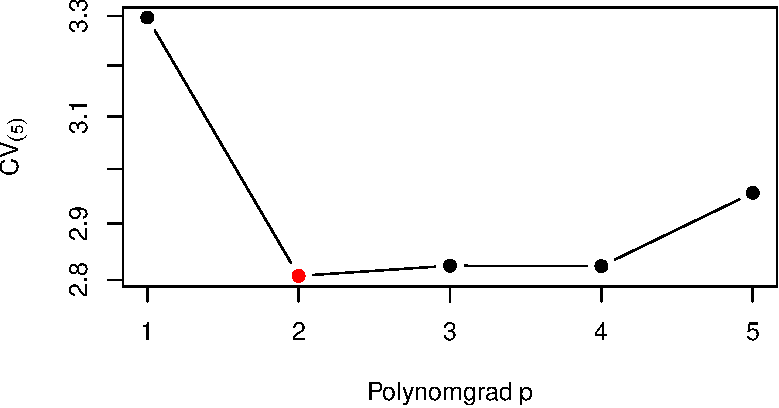
\includegraphics[width=0.9\linewidth]{Computational_Statistics_Script_files/figure-latex/AutoCV-1} \end{center}

Auch der \(5\)-fache Kreuzvalidierungswert \(\operatorname{CV}_{(5)}\) ist lediglich eine zufallsbehaftete Schätzung des unbekannten mittleren quadratischen Prädiktionsfehlers \(E[(Y-\hat{Y})^2]\). Um eine Idee von der Präzision und Stabilität der Modellauswahl mittels der Minimierung von \(\operatorname{CV}_{(5)}\) zu bekommen, können wir die zufälligen, \(5\)-fachen Aufteilungen der Daten in Trainins- und Validierungsdaten wiederholen und den Effekt alternativer Datenaufteilungen betrachten. Abbildung \ref{fig:AutoCV2} zeigt, dass die Minimierung des Kreuzvalidierungswertes \(\operatorname{CV}_{(5)}\) auch in Wiederholungen häufig das Modell mit Polynomgrad \(p=2\) auswählt. Der Polynomgrad \(p=2\) scheint also eine vertauenswürde Modellauswahl darzustellen.\\

\begin{figure}[h]

{\centering 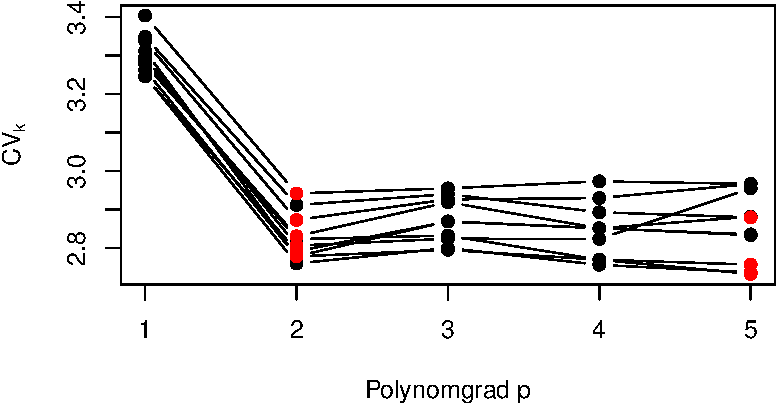
\includegraphics[width=0.9\linewidth]{Computational_Statistics_Script_files/figure-latex/AutoCV2-1} 

}

\caption{Zehn verschiedene $\operatorname{CV}_{(k)}$-Berechnungen basierend auf zehn verschiedenen, zufälligen Wiederholungen der $5$-fachen Kreuzvalidierung.}\label{fig:AutoCV2}
\end{figure}

Das Polynomregressionsmodell mit \(p=2\) stellt also ein gutes Prädiktionsmodell dar. Wir verwenden nun dieses Modell, um nach auffälligen Unterschiedenen in den herstellerseitigen Verbrauchsangaben \(y_i\) und unseren Prädiktionen zu suchen. Gerade \textbf{stark negative Residuen} \(y_i-\hat{y}_i\) sind verdächtig, da es auf eine Schönung der Verbrauchsangaben hindeuten könnte.

Folgender R-Code schätzt zunächst das Polynomregressionsmodell mit \(p=2\), berechnet dann die Residuen \(y_i-\hat{y}_i\) und veranschaulicht die größte negative Abweichung in Abbildung \ref{fig:mazda}.

\begin{Shaded}
\begin{Highlighting}[]

\NormalTok{p }\OtherTok{\textless{}{-}} \DecValTok{2}
\NormalTok{poly\_fit }\OtherTok{\textless{}{-}} \FunctionTok{lm}\NormalTok{(Verbrauch }\SpecialCharTok{\textasciitilde{}}
                   \FunctionTok{poly}\NormalTok{(Gewicht,        }\AttributeTok{degree =}\NormalTok{ p, }\AttributeTok{raw =} \ConstantTok{TRUE}\NormalTok{) }\SpecialCharTok{+}
                   \FunctionTok{poly}\NormalTok{(PS,             }\AttributeTok{degree =}\NormalTok{ p, }\AttributeTok{raw =} \ConstantTok{TRUE}\NormalTok{) }\SpecialCharTok{+}
                   \FunctionTok{poly}\NormalTok{(Hubraum,        }\AttributeTok{degree =}\NormalTok{ p, }\AttributeTok{raw =} \ConstantTok{TRUE}\NormalTok{),}
                 \AttributeTok{data=}\NormalTok{Auto\_df)}

\FunctionTok{par}\NormalTok{(}\AttributeTok{mar=}\FunctionTok{c}\NormalTok{(}\FloatTok{5.1}\NormalTok{, }\FloatTok{5.1}\NormalTok{, }\FloatTok{4.1}\NormalTok{, }\FloatTok{2.1}\NormalTok{))}
\FunctionTok{plot}\NormalTok{(}\AttributeTok{y =} \FunctionTok{resid}\NormalTok{(poly\_fit), }\AttributeTok{x =} \FunctionTok{fitted}\NormalTok{(poly\_fit), }
     \AttributeTok{ylab =} \FunctionTok{expression}\NormalTok{(}\StringTok{"Residuen:"}\SpecialCharTok{\textasciitilde{}}\NormalTok{y[i] }\SpecialCharTok{{-}} \FunctionTok{hat}\NormalTok{(y)[i]), }
     \AttributeTok{xlab =} \FunctionTok{expression}\NormalTok{(}\StringTok{"Prädiktionen:"}\SpecialCharTok{\textasciitilde{}}\FunctionTok{hat}\NormalTok{(y)[i]),}
     \AttributeTok{main=}\StringTok{"Größte negative Abweichung der Verbrauchsangabe"}\NormalTok{)}
\NormalTok{slct }\OtherTok{\textless{}{-}} \FunctionTok{order}\NormalTok{(}\FunctionTok{abs}\NormalTok{(}\FunctionTok{resid}\NormalTok{(poly\_fit)), }\AttributeTok{decreasing =} \ConstantTok{TRUE}\NormalTok{)[}\DecValTok{4}\NormalTok{]}
\FunctionTok{points}\NormalTok{(}\AttributeTok{y =} \FunctionTok{resid}\NormalTok{(poly\_fit)[slct], }\AttributeTok{x =} \FunctionTok{fitted}\NormalTok{(poly\_fit)[slct], }
       \AttributeTok{col =} \StringTok{"red"}\NormalTok{, }\AttributeTok{bg =} \StringTok{"red"}\NormalTok{, }\AttributeTok{pch =} \DecValTok{21}\NormalTok{)}
\FunctionTok{text}\NormalTok{(}\AttributeTok{y =} \FunctionTok{resid}\NormalTok{(poly\_fit)[slct], }\AttributeTok{x =} \FunctionTok{fitted}\NormalTok{(poly\_fit)[slct], }
     \AttributeTok{labels =} \StringTok{"Mazda RX{-}3 (1973)"}\NormalTok{, }\AttributeTok{pos =} \DecValTok{2}\NormalTok{)}
\end{Highlighting}
\end{Shaded}

\begin{figure}[h]

{\centering 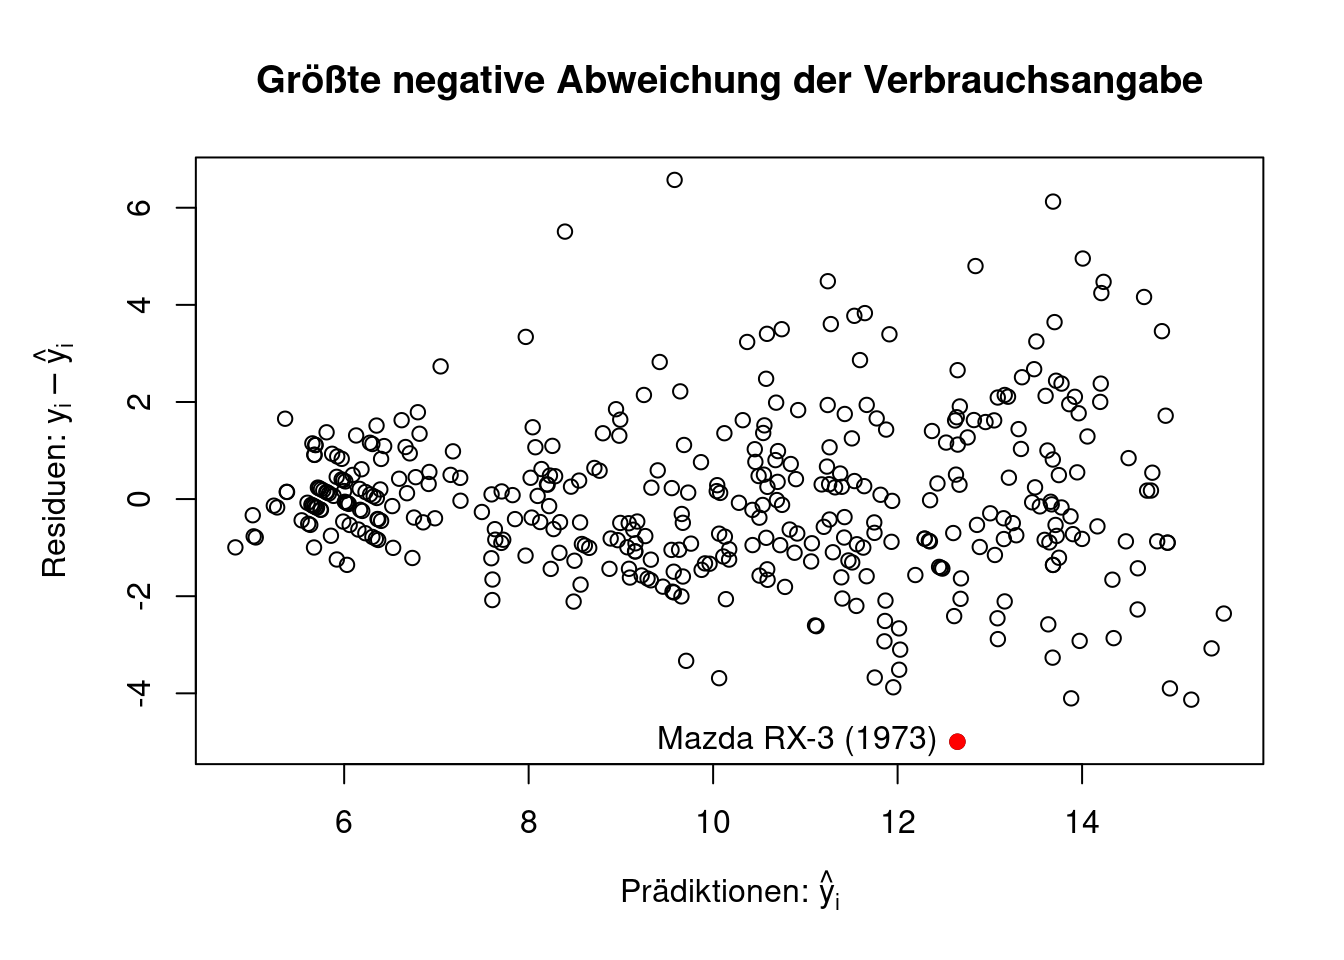
\includegraphics[width=0.9\linewidth]{Computational_Statistics_Script_files/figure-latex/mazda-1} 

}

\caption{Polynomregression im Anwendungsbeispiel zum Benzinverbrauch. Die größte negative Abweichung ist der Mazda RX-3 von 1973.}\label{fig:mazda}
\end{figure}

\begin{Shaded}
\begin{Highlighting}[]
\FunctionTok{par}\NormalTok{(}\AttributeTok{mar=}\FunctionTok{c}\NormalTok{(}\FloatTok{5.1}\NormalTok{, }\FloatTok{4.1}\NormalTok{, }\FloatTok{4.1}\NormalTok{, }\FloatTok{2.1}\NormalTok{))}
\end{Highlighting}
\end{Shaded}

Wir haben hier tatsächlich einen besonderen Fall gefunden. Der Mazda RX-3 (1973) (Abbildung \ref{fig:mazda2}) lief mit einem ungewöhnlich sparsamen \href{https://de.wikipedia.org/wiki/Wankelmotor}{Wankelmotor}. Dieser Motor war so ungewöhnlich, dass es vielerlei \href{https://nepis.epa.gov/Exe/ZyNET.exe/9100X47O.txt?ZyActionD=ZyDocument\&Client=EPA\&Index=Prior\%20to\%201976\&Docs=\&Query=\&Time=\&EndTime=\&SearchMethod=1\&TocRestrict=n\&Toc=\&TocEntry=\&QField=\&QFieldYear=\&QFieldMonth=\&QFieldDay=\&UseQField=\&IntQFieldOp=0\&ExtQFieldOp=0\&XmlQuery=\&File=D\%3A\%5CZYFILES\%5CINDEX\%20DATA\%5C70THRU75\%5CTXT\%5C00000016\%5C9100X47O.txt\&User=ANONYMOUS\&Password=anonymous\&SortMethod=h\%7C-\&MaximumDocuments=1\&FuzzyDegree=0\&ImageQuality=r75g8/r75g8/x150y150g16/i425\&Display=hpfr\&DefSeekPage=x\&SearchBack=ZyActionL\&Back=ZyActionS\&BackDesc=Results\%20page\&MaximumPages=1\&ZyEntry=2\#}{Streitigkeiten} um die Verbrauchsangaben gab.

\hypertarget{ende-1}{%
\section{Ende}\label{ende-1}}

  \bibliography{book.bib,packages.bib}

\end{document}
